%%%%%%%%%%%%%%%%%%%%%%%%%%%%%%%%%%%%%%%%%%%%%%%%%%%%%%%%%%%%%%%%%%%%%%%%%%%%%%%%
%%                                                                            %%
%%                                                                            %%
%% An example for writting your thesis using LaTeX                            %%
%% Original version and development work by Luis Costa, changes to the text   %% 
%% in the Finnish template by Perttu Puska.                                   %%
%% Support for Swedish added 15092014                                         %%
%% PDF/A-b support added on 15092017                                          %%
%% PDF/A-2 support added on 24042018                                          %%
%%                                                                            %%
%% This example consists of the files                                         %%
%%         thesistemplate.tex (version 3.20) (for text in English)            %%
%%         opinnaytepohja.tex (version 3.20) (for text in Finnish)            %%
%%         kandidatarbetsbotten.tex (version 1.00) (for text in Swedish)      %%
%%         aaltothesis.cls (versio 3.20)                                      %%
%%         kuva1.eps (graphics file)                                          %%
%%         kuva2.eps (graphics file)                                          %%
%%         kuva1.jpg (graphics file)                                          %%
%%         kuva2.jpg (graphics file)                                          %%
%%         kuva1.png (graphics file)                                          %%
%%         kuva2.png (graphics file)                                          %%
%%         kuva1.pdf (graphics file)                                          %%
%%         kuva2.pdf (graphics file)                                          %%
%%                                                                            %%
%%                                                                            %%
%% Typeset in Linux either with                                               %%
%% pdflatex: (recommended method)                                             %%
%%             $ pdflatex thesistemplate                                      %%
%%             $ pdflatex thesistemplate                                      %%
%%                                                                            %%
%%   The result is the file thesistemplate.pdf that is PDF/A compliant, if    %%
%%   you have chosen the proper \documenclass options (see comments below)    %%
%%   and your included graphics files have no problems.
%%                                                                            %%
%% Or                                                                         %%
%% latex: (this method is not recommended)                                    %%
%%             $ latex thesistemplate                                         %%
%%             $ latex thesistemplate                                         %%
%%                                                                            %%
%%   The result is the file thesistemplate.dvi, which is converted to ps      %%
%%   format as follows:                                                       %%
%%                                                                            %%
%%             $ dvips thesistemplate -o                                      %%
%%                                                                            %%
%%   and then to pdf as follows:                                              %%
%%                                                                            %%
%%             $ ps2pdf thesistemplate.ps                                     %%
%%                                                                            %%
%%   This pdf file is not PDF/A compliant. You must must make it so using,    %%
%%   e.g., Acrobat Pro or PDF-XChange.                                        %%
%%                                                                            %%
%%                                                                            %%
%% Explanatory comments in this example begin with the characters %%, and     %%
%% changes that the user can make with the character %                        %%
%%                                                                            %%
%%%%%%%%%%%%%%%%%%%%%%%%%%%%%%%%%%%%%%%%%%%%%%%%%%%%%%%%%%%%%%%%%%%%%%%%%%%%%%%%
%%%%%%%%%%%%%%%%%%%%%%%%%%%%%%%%%%%%%%%%%%%%%%%%%%%%%%%%%%%%%%%%%%%%%%%%%%%%%%%%
%%
%% WHAT is PDF/A
%%
%% PDF/A is the ISO-standardized version of the pdf. The standard's goal is to
%% ensure that he file is reproducable even after a long time. PDF/A differs
%% from pdf in that it allows only those pdf features that support long-term
%% archiving of a file. For example, PDF/A requires that all used fonts are
%% embedded in the file, whereas a normal pdf can contain only a link to the
%% fonts in the system of the reader of the file. PDF/A also requires, among
%% other things, data on colour definition and the encryption used.
%% Currently three PDF/A standards exist:
%% PDF/A-1: based on PDF 1.4, standard ISO19005-1, published in 2005.
%%          Includes all the requirements essential for long-term archiving.
%% PDF/A-2: based on PDF 1.7, standard ISO19005-2, published in 2011.
%%          In addition to the above, it supports embedding of OpenType fonts,
%%          transparency in the colour definition and digital signatures.
%% PDF/A-3: based on PDF 1.7, standard ISO19005-3, published in 2012.
%%          Differs from the above only in that it allows embedding of files in
%%          any format (e.g., xml, csv, cad, spreadsheet or wordprocessing
%%          formats) into the pdf file.
%% PDF/A-1 files are not necessarily PDF/A-2 -compatible and PDF/A-2 are not
%% necessarily PDF/A-1 -compatible.
%% All of the above PDF/A standards have two levels:
%% b: (basic) requires that the visual appearance of the document is reliably
%%    reproduceable.
%% a (accessible) in addition to the b-level requirements, specifies how
%%   accessible the pdf file is to assistive software, say, for the physically
%%   impaired.
%% For more details on PDF/A, see, e.g., https://en.wikipedia.org/wiki/PDF/A
%%
%%
%% WHICH PDF/A standard should my thesis conform to?
%%
%% Primarily to the PDF/A-1b standard. All the figures and graphs typically
%% use in thesis work do not require transparency features, a basic '2-D'
%% visualisation suffices. The font to be used are specified in this template
%% and they should not be changed. However, if you have figures where
%% transparency characteristics matter, use the PDF/A-2b standard. Do not use
%% the PDF/A-3b standard for your thesis.
%%
%%
%% WHAT graphics format can I use to produce my PDF/A compliant file?
%%
%% When using pdflatex to compile your work, use jpg, png or pdf files. You may
%% have PDF/A compliance problems with figures in pdf format. Do not use PDF/A
%% compliant graphics files.
%% If you decide to use latex to compile your work, the only acceptable file
%% format for your figure is eps. DO NOT use the ps format for your figures.

%% USE one of these:
%% * the first when using pdflatex, which directly typesets your document in the
%%   chosen pdf/a format and you want to publish your thesis online,

%% * the second when you want to print your thesis to bind it, or
%% * the third when producing a ps file and a pdf/a from it.
%%
\documentclass[english, 12pt, a4paper, sci, utf8, a-1b, online]{aaltothesis}
%\documentclass[english, 12pt, a4paper, elec, utf8, a-1b]{aaltothesis}
%\documentclass[english, 12pt, a4paper, elec, dvips, online]{aaltothesis}

%% Use the following options in the \documentclass macro above:
%% your school: arts, biz, chem, elec, eng, sci
%% the character encoding scheme used by your editor: utf8, latin1
%% thesis language: english, finnish, swedish
%% make an archiveable PDF/A-1b or PDF/A-2b compliant file: a-1b, a-2b
%%                    (with pdflatex, a normal pdf containing metadata is
%%                     produced without the a-*b option)
%% typeset in symmetric layout and blue hypertext for online publication: online
%%            (no option is the default, resulting in a wide margin on the
%%             binding side of the page and black hypertext)
%% two-sided printing: twoside (default is one-sided printing)
%%

\usepackage{graphicx}
\usepackage{listings}

%% Math fonts, symbols, and formatting; these are usually needed
\usepackage{amsfonts,amssymb,amsbsy,amsmath}

%% Change the school field to specify your school if the automatically set name
%% is wrong
% \university{aalto-yliopisto}
% \school{Sähkötekniikan korkeakoulu}

%% Edit to conform to your degree programme
%%
\degreeprogram{Master's Programme in ICT Innovation}
%%

%% Your major
%%
\major{Data Science}
%%

%% Major subject code
%%
\code{SCI3115}
%%
 
%% Choose one of the three below
%%
%\univdegree{BSc}
\univdegree{MSc}
%\univdegree{Lic}
%%

%% Your name (self explanatory...)
%%
\thesisauthor{Cristian M. Abrante Dorta}
%%

%% Your thesis title comes here and possibly again together with the Finnish or
%% Swedish abstract. Do not hyphenate the title, and avoid writing too long a
%% title. Should LaTeX typeset a long title unsatisfactorily, you mght have to
%% force a linebreak using the \\ control characters.
%% In this case...
%% Remember, the title should not be hyphenated!
%% A possible "and" in the title should not be the last word in the line, it
%% begins the next line.
%% Specify the title again without the linebreak characters in the optional
%% argument in box brackets. This is done because the title is part of the 
%% metadata in the pdf/a file, and the metadata cannot contain linebreaks.
%%
\thesistitle{Domain-Oriented Microservices Gateway monitoring using big data techniques}
%\thesistitle[Title of the thesis]{Title of\\ the thesis}
%%

%%
\place{Otaniemi, Espoo}
%%

%% The date for the bachelor's thesis is the day it is presented
%%
\date{\today}
%%

%% Thesis supervisor
%% Note the "\" character in the title after the period and before the space
%% and the following character string.
%% This is because the period is not the end of a sentence after which a
%% slightly longer space follows, but what is desired is a regular interword
%% space.
%%
\supervisor{Prof.\ Hong-Linh Truong}
%%

%% Advisor(s)---two at the most---of the thesis. Check with your supervisor how
%% many official advisors you can have.
%%
\advisor{Msc.\ Teemu Sidoroff}
%%

%% Aaltologo: syntax:
%% \uselogo{aaltoRed|aaltoBlue|aaltoYellow|aaltoGray|aaltoGrayScale}{?|!|''}
%% The logo language is set to be the same as the thesis language.
%%
\uselogo{aaltoRed}{''}
%%

%% The English abstract:
%% All the details (name, title, etc.) on the abstract page appear as specified
%% above.
%% Thesis keywords:
%% Note! The keywords are separated using the \spc macro
%%
\keywords{FILL KEYWORDS FOR THE THESIS}
%%

%% The abstract text. This text is included in the metadata of the pdf file as well
%% as the abstract page.
%%
\thesisabstract{
FILL THE ABSTRACT OF THE THESIS
}

%% Copyright text. Copyright of a work is with the creator/author of the work
%% regardless of whether the copyright mark is explicitly in the work or not.
%% You may, if you wish, publish your work under a Creative Commons license (see
%% creaticecommons.org), in which case the license text must be visible in the
%% work. Write here the copyright text you want. It is written into the metadata
%% of the pdf file as well.
%% Syntax:
%% \copyrigthtext{metadata text}{text visible on the page}
%% 
%% In the macro below, the text written in the metadata must have a \noexpand
%% macro before the \copyright special character, and macros (\copyright and
%% \year here) must be separated by the \ character (space chacter) from the
%% text that follows. The macros in the argument of the \copyrighttext macro
%% automatically insert the year and the author's name. (Note! \ThesisAuthor is
%% an internal macro of the aaltothesis.cls class file).
%% Of course, the same text could have simply been written as
%% \copyrighttext{Copyright \noexpand\copyright\ 2018 Eddie Engineer}
%% {Copyright \copyright{} 2018 Eddie Engineer}
%%
\copyrighttext{Copyright \noexpand\copyright\ \number\year\ \ThesisAuthor}
{Copyright \copyright{} \number\year{} \ThesisAuthor}

%% You can prevent LaTeX from writing into the xmpdata file (it contains all the 
%% metadata to be written into the pdf file) by setting the writexmpdata switch
%% to 'false'. This allows you to write the metadata in the correct format
%% directly into the file thesistemplate.xmpdata.
%\setboolean{writexmpdatafile}{false}

\colorlet{punct}{red!60!black}
\definecolor{background}{HTML}{EEEEEE}
\definecolor{delim}{RGB}{20,105,176}
\colorlet{numb}{magenta!60!black}
\definecolor{dkgreen}{rgb}{0,0.6,0}
\definecolor{ltgray}{rgb}{0.5,0.5,0.5}

\lstdefinelanguage{json}{
    basicstyle=\normalfont\ttfamily,
    numbers=left,
    numberstyle=\scriptsize,
    stepnumber=1,
    numbersep=8pt,
    showstringspaces=false,
    breaklines=true,
    frame=lines,
    backgroundcolor=\color{background},
    literate=
     *{0}{{{\color{numb}0}}}{1}
      {1}{{{\color{numb}1}}}{1}
      {2}{{{\color{numb}2}}}{1}
      {3}{{{\color{numb}3}}}{1}
      {4}{{{\color{numb}4}}}{1}
      {5}{{{\color{numb}5}}}{1}
      {6}{{{\color{numb}6}}}{1}
      {7}{{{\color{numb}7}}}{1}
      {8}{{{\color{numb}8}}}{1}
      {9}{{{\color{numb}9}}}{1}
      {:}{{{\color{punct}{:}}}}{1}
      {,}{{{\color{punct}{,}}}}{1}
      {\{}{{{\color{delim}{\{}}}}{1}
      {\}}{{{\color{delim}{\}}}}}{1}
      {[}{{{\color{delim}{[}}}}{1}
      {]}{{{\color{delim}{]}}}}{1},
}

\lstdefinelanguage{JavaScript}{
  keywords={typeof, new, true, false, catch, function, return, null, catch, switch, var, if, in, while, do, else, case, break},
  keywordstyle=\color{blue}\bfseries,
  ndkeywords={class, export, boolean, throw, implements, import, this},
  ndkeywordstyle=\color{darkgray}\bfseries,
  identifierstyle=\color{black},
  sensitive=false,
  comment=[l]{//},
  morecomment=[s]{/*}{*/},
  commentstyle=\color{purple}\ttfamily,
  stringstyle=\color{red}\ttfamily,
  morestring=[b]',
  morestring=[b]"
}

\lstset{
  	backgroundcolor=\color{background},
  	basicstyle=\normalfont\ttfamily,
  	breakatwhitespace=false,
  	breaklines=true,
  	captionpos=b,
  	commentstyle=\color{dkgreen},
  	deletekeywords={...},
  	escapeinside={\%*}{*)},
  	extendedchars=true,
  	frame=single,
  	keepspaces=true,
  	keywordstyle=\color{blue},
  	language=SQL,
  	morekeywords={*,modify,MODIFY,...},
  	numbers=left,
  	numbersep=15pt,
  	numberstyle=\tiny,
  	rulecolor=\color{ltgray},
  	showspaces=false,
  	showstringspaces=false, 
  	showtabs=false,
  	stepnumber=1,
  	tabsize=4,
  	title=\lstname
}

%% All that is printed on paper starts here
%%
\begin{document}

%% Create the coverpage
%%
\makecoverpage

%% Typeset the copyright text.
%% If you wish, you may leave out the copyright text from the human-readable
%% page of the pdf file. This may seem like a attractive idea for the printed
%% document especially if "Copyright (c) yyyy Eddie Engineer" is the only text
%% on the page. However, the recommendation is to print this copyright text.
%%
\makecopyrightpage

%% Note that when writting your thesis in English, place the English abstract
%% first followed by the possible Finnish or Swedish abstract.

%% Abstract text
%% All the details (name, title, etc.) on the abstract page appear as specified
%% above.
%%
\begin{abstractpage}[english]
  \abstracttext{}
\end{abstractpage}

%% The text in the \thesisabstract macro is stored in the macro \abstractext, so
%% you can use the text metadata abstract directly as follows:
%%
%\begin{abstractpage}[english]
%	\abstracttext{}
%\end{abstractpage}

%% Force a new page so that the possible Finnish or Swedish abstract does not
%% begin on the same page
%%
\newpage

%% Preface
%%
%% This section is optional. Remove it if you do not want a preface.
\mysection{Acknowledgements}

FILL THE AKNOWLEDGEMENTS SECTION.

\vspace{5cm}
Otaniemi, \today

\vspace{5mm}
{\hfill Cristian M.\ Abrante Dorta \hspace{1cm}}

%% Force a new page after the preface
%%
\newpage


%% Table of contents. 
%%
\thesistableofcontents


%% Symbols and abbreviations
\mysection{Abbreviations}

\begin{tabular}{ll}
SOA          & Service oriented architecture \\
DOMA         & Domain-oriented microservices architecture \\
WSDL         & Web Service Deskcription Language \\
SOAP         & Simple Object Acess Protocol \\
RPC          & Remote Procedure Call \\
REP          & Request Execution Path \\
RFC          & Request for comments \\
BQ           & BigQuery \\
VCS          & Version Control System\\
JSON         & JavaScript Object Notation\\
UI           & User Interface\\
PR           & Pull Request\\
GCP          & Google Cloud Plattform\\
CI           & Continuous Integration\\
CI/CD        & Continuous Integration and Continuous Deployment\\
gRPC         & Google Remote Procedure Call\\

\end{tabular}


%% \clearpage is similar to \newpage, but it also flushes the floats (figures
%% and tables).
%%
\cleardoublepage

%% Text body begins. Note that since the text body is mostly in Finnish the
%% majority of comments are also in Finnish after this point. There is no point
%% in explaining Finnish-language specific thesis conventions in English.
%% This text will be translated to English soon.
%%

%%
%% Introduction.
%% In this part I have to state why the thesis is relevant.
%% Just check the thesis proposal.
%% 
\section{Introduction}

%% For the introduction I guess it can be mostly copied from the thesis proposal,
%% anyway one of the last sections to write.

Over the past few years, there has been debate on how to properly organize and deploy service-oriented architectures. One of the software architecture patterns that has gained the most popularity today is microservices \cite{MicroservicesAdoption}. Many large, medium and even small software companies have adopted this architecture because of its enormous benefits compared to traditional, monolithic software applications.\\

Microservices are an extension of service-oriented architecture. The main objective is that each of these microservices provides a well-defined and clear scope of functionalities, which can be accessed by another microservice using \textit{remote procedure calls} \cite{nelson1981remote}. The main advantage of this pattern is that it can be established clear ownership of each microservice by different teams where they are responsible for the development, maintenance, and deployment. This is a clear advantage over the classic monolithic architecture, since in these, although the development tasks may be divided among different teams, the deployment of a single functionality involves the deployment of the entire system, which is then prone to cause major problems that can lead to the complete shutdown of the application.\\

Although the microservices architecture represents a step forward in the design of software systems, it also has some drawbacks compared to monolithic architectures, such as performance. In a traditional monolithic application subroutine calls are something that can be solved within the same process and machine, however, in microservices, the call has to be made over the network, which is something that may eventually introduce some execution delays. Apart from this, there is another problem faced by microservices architectures, which is the orchestration of thousands of different microservices, when dealing with enterprises operating on a large scale. In this case, any problem caused by one microservice can spread across many of them, and engineers have to debug calls coming from a huge stack of different services, which is something that can be challenging and time-consuming.\\

In order to provide an scope that would simplify the maintenance of the microservices set, many companies had adopted the \textbf{Domain Oriented Microservices Architecture} pattern \cite{DOMAUber}. Using this architecture, many microservices can be grouped within a logical division, called Domain, that fits the needs of the enterprise. To isolate the domains and make them easier to maintain and debug, one approach which can be applied is to create a common gateway that exposes the domain's interface (usually as routes that can be called with different HTTP methods). Apart from being the single point of entry for specific domains, the gateway can also provide different high-level responsibilities, such as authentication, routing, rate limiting, load balancing, etc. This pattern has been widely adopted by companies operating on a large scale, such as Uber \cite{GatewayUber} or Unity Technologies (Figure \ref{fig:unity-acquire-domain}).\\

\begin{figure}[h]
    \centering
    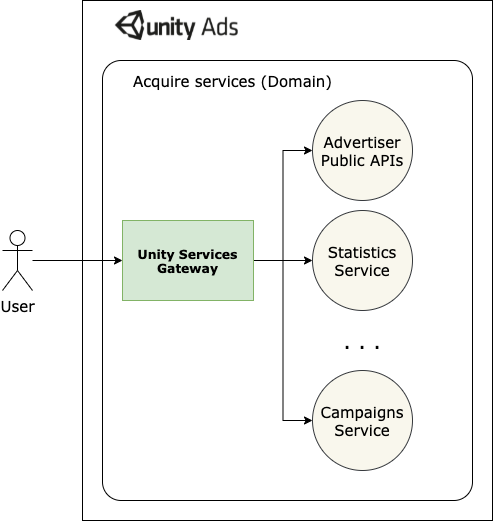
\includegraphics[scale=0.3]{src/proposal/img/unity-services-diagram.png}
    \caption{Domain-oriented microservices architecture structure in Unity Technologies}
    \label{fig:unity-acquire-domain}
\end{figure}

The gateway is in itself another microservice, consequently the error monitoring of it is a crucial task for maintenance the overall health of the system. About microservices logging and monitoring there is already a well established action framework \cite{MicroservicesBestPractices}, which can be summarized as the storage of a log entry in a centralized server (for example Google Cloud or Amazon Web Services) for each request or error that it is produced in the system. Usually that is enough for tracing back each of the requests that the system is receiving.\\

In the particular case of the \textbf{Unity Services Gateway}, which is the entry point of the acquire domain of Unity technologies, there are some questions raised about the high-level responsibilities of the gateway by project managers or development teams, such as: \textit{what users or organizations are hitting our rate limits?} \textit{What is the amount and frequency of authentication errors our system is having?}.\\

The answers to those questions are relevant because some actions can be taking against malicious users which are doing too many queries to the system or directly some organizations can be contacted to check if their integration with the APIs that the company provides are working properly. Nevertheless, the current log setup, which is the classical microservices logging framework \cite{MicroservicesBestPractices}, is not enough for answering those questions. This is mainly due to the fact that they only store the minimal piece of information required to trace back the request but do not contain complex fields, such as organization ids, paths for the request, rate limit quotas exceeded, etc.\\

One might think that simply by extending the logs entry to contain more information is enough for solving this problem, nevertheless this simple approach is not effective due to some reasons. The first one is that the data needed for solving those questions has to be extracted from different sources, which is something that it is reasonable to do when dealing with errors but can not be generalized to all logs entries as would dramatically increase the processing time of the requests in a system that is receiving thousands of request per seconds. The second reason is that the logging tool is shared among many microservices, so none of them has to worry in how to communicate with the cloud provider, this is why it is better to keep simple the amount of fields that the logs are storing. The final reason is the single responsibility principle, as it seems sensible to separate the data store that would keep complex error fields that would solve high-level questions from the actual log registry that would keep track of the requests.\\

Taking this into account, the objective of this thesis can be defined as determine the best way to monitor the errors produced by the high-level responsibilities of a Domain Oriented Microservice Architecture gateway.

\subsection{Contributions}

% Explain the contributions introduced in that thesis.

This thesis proposes a monitoring framework for a Domain-Oriented Microservice Architecture gateway that allows stakeholders to observe the errors that the gateway is producing when performing its high-level operations. Particularly, the introduced framework offers the following characteristics:

\begin{itemize}
    \item Definition of a format that matches the high-level responsibilities that the DOMA gateway has to fulfill for every endpoint it exposes.
    \item Definition of an extensible error format that will be emitted by the gateway and stored on a data warehouse for the visualization and analysis afterward.
    \item Creation of a cloud-agnostic data pipeline that transmits the errors from the emission on the gateway to the data storage.
    \item Creation of a visualization dashboard that will retrieve the error data and visualize it in a convenient structure.
\end{itemize}

This framework is created for the particular case of the Unity Services Gateway, the DOMA gateway for Unity technologies, a highly-available service that handles thousands of requests per second, and that it is managed by a growing team of engineers located in different parts of the world.

\subsection{Structure of the thesis}

This thesis is divided into seven sections. The first one is the introduction, where the proposed contributions are highlighted. Section \ref{sec:background} is the background, where there is an overview of the company's architecture and a definition of the problem that will be tackled. Section \ref{sec:requirements-eng} covers requirements engineering, which defines and establishes the project's scope according to its stakeholders. Subsequently, section \ref{sec:literature-review} will give a literature review, introducing the different software architectures used nowadays, primarily focusing on DOMA. Furthermore, there is a high-level view of other industry-standard solutions for API gateways. Then, section \ref{sec:technical-solution} will explain the technical solution and all the created artifacts for the proposed framework. Also, section \ref{sec:evaluation} will explain the followed evaluation process, especially compared with other industry-standard solutions. Finally, in section \ref{sec:consclussion}, some conclusions to this work will be offered in addition to future work that can be done in this regard.

% Easy section, it can be mostly written now.

%% Leave page number of the first page empty
\thispagestyle{empty}

\clearpage
\section{Background}
\label{sec:background}

%% The objective of the background section is to give a business context to explain where the problem come from.

This section describes all the necessary background to understand the problem that this thesis seeks to address. In the first subsection, a brief introduction is made about the company and the business environment in which it operates, and in the second subsection, the problem is framed from different points of view, taking into account the various stakeholders involved.

\subsection{Company description}

%% Describe Unity technologies as a company.
%% Describe Unity Acquire architecture.
%% Describe Unity Acquire Microservices architecture.
%% Describe Unity Services gateway and why it is needed.

To better understand the project, it is essential to present the company where it has been developed. This thesis is done in collaboration with Unity Technologies \cite{UnityTechnologies}, a multinational company based in the United States. The company's main product is the Unity game engine \cite{haas2014history}, an industry standard for game and 3D content development  \cite{nicoll2019unity}.\\

Although the game engine is the most famous product offered by the company, it is not the only source of revenue, and it is not enough to understand its business model. This is mainly because the company's value proposition can be summarized as: \textit{"Create a platform for creators to develop, execute and monetize their content"} \cite{UnityBusinessModel}. To realize this value proposition, the company has established two organizational departments that offer various products to its users.\\

\begin{figure}[h]
    \centering
    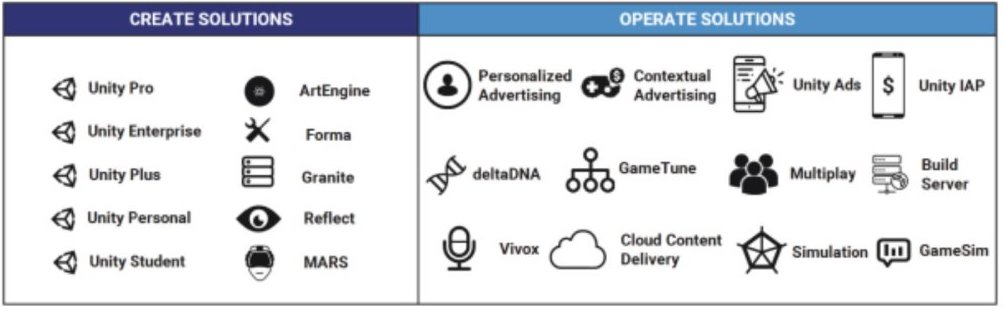
\includegraphics[scale=0.3]{src/thesis/img/background/unity-division.jpg}
    \caption{Products offered in the two organizational divisions of Unity Technologies}
    \label{fig:unity-solutions}
\end{figure}

\begin{itemize}
    \item \textbf{Create solutions}: The main functionality of this product suite is to offer a set of tools that allows users to produce all kinds of 3D content. The business model of this division consists of a subscription-based model for the different versions of the Unity Editor.
    \item \textbf{Operate solutions}: The goal of the products categorized in this section is to enable creators to run a successful business from their 3D content. This is the organizational section that contains UnityAds, the product on which this thesis project was developed.
\end{itemize}

\subsubsection{UnityAds}

To understand UnityAds correctly, first, it is essential to clarify the concept of \textbf{online advertising network} \cite{goldfarb2011online} \cite{schmeiser2016online}. An advertising network is a type of business or service whose purpose is to connect advertisers, who are individuals who want to display advertisements for the products they intend to sell, with publishers, who are individuals who can provide space to place such advertisements, and who usually reach a certain level of audience. The original definition of advertisement network was really tied to newspapers, magazines, and television, but in recent years, it has been extended to online services \cite{ha2008online}. In that sense, UnityAds proposes a new innovative business idea because it is an ad-hoc advertisement network for the game industry. In a nutshell, UnityAds allows game developers to show ads about their games in other games and place advertisements of other games in theirs \cite{chu2013iad}. As can be seen, by using UnityAds, the same game developer can be publisher and advertiser simultaneously, melting both roles.\\

\begin{figure}[h]
    \centering
    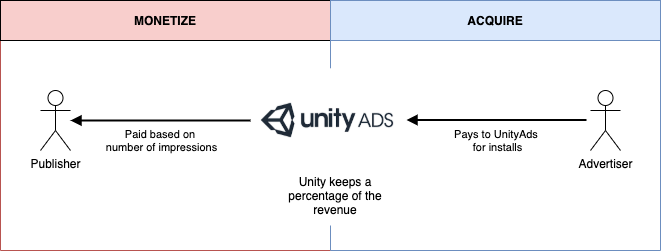
\includegraphics[scale=0.4]{src/thesis/img/background/unity-ads.png}
    \caption{Simplified structure of UnityAds}
    \label{fig:background:unity-ads}
\end{figure}

Figure \ref{fig:background:unity-ads} shows the two aspects that make up the advertising network: \textbf{Acquire} and \textbf{Monetize}. The terms correspond to the classic definition of publisher and advertiser but translated into the gaming industry terminology.

\begin{itemize}
    \item \textbf{Monetize unit}: This section includes all the tools provided to game developers to monetize their games, in addition to all the technical solutions needed to deliver an ad to the mobile game that has a publisher space.
    \item \textbf{Acquire unit}: This set of tools includes all the products that help advertisers acquire new users who can install the games they advertise on the network.
\end{itemize}

Although this overall context of UnityAds was essential to understand the big picture, only the Acquire unit is considered in the following sections, as the thesis project focuses on it.

\subsubsection{Acquire architecture overview}
\label{sec:acquire-architecture}

This section covers the architecture overview for the acquire unit of UnityAds. It is important to note that many details of the architecture will not be explained in-depth to respect the company's privacy.\\

The architecture of UnityAds has changed dramatically over the past decade. Initially, the ad network was developed by a Finnish startup, Applifier, acquired by Unity Technologies in 2014 \cite{UnityBuyApplifier}. The initial architecture of the Applifier ad network can be seen in figure \ref{fig:background:applifier-architecture}.

\begin{figure}[h]
    \centering
    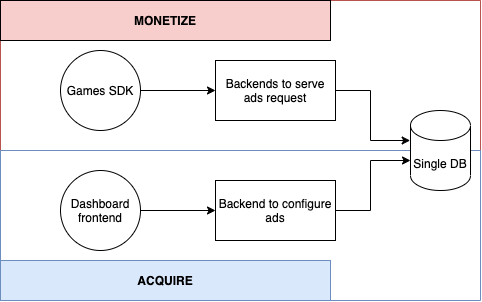
\includegraphics[scale=0.4]{src/thesis/img/background/applifier-unityads-architecture.png}
    \caption{Diagram for the initial architecture of Applifier}
    \label{fig:background:applifier-architecture}
\end{figure}

This almost \textit{monolithic architecture} \cite{de2019monolithic} was convenient for a small engineering team to introduce changes to it, which allowed them to achieve a solid customer base prior to the Unity acquisition \cite{ApplifierCustomers}. But when scalability started to become a fundamental requirement, there were some pain points they had to address. On the one hand, the database was the junction point between the services and the mechanism they used to communicate, which was limiting and error-prone, and on the other hand, this architecture was not suitable to be managed by a growing team of engineers. Due to this, migration started into a microservices-oriented architecture (Section \ref{sec:microservices-architecture}). This means that now the database is not the single point of communication, and each of the services would need an independent database to store the data they needed to operate. The acquire and monetize units can easily be decoupled using that paradigm, and different teams could work independently. This initiative led the company to its current setup, which can be observed in figure \ref{fig:background:acquire-architecture}.\\

\begin{figure}[h!]
    \centering
    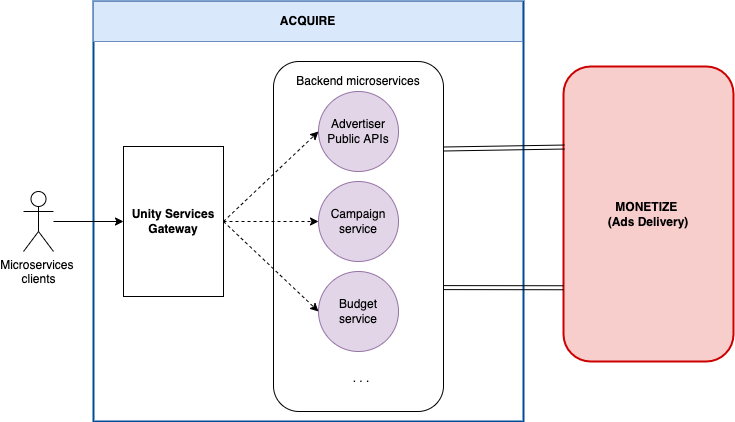
\includegraphics[scale=0.3]{src/thesis/img/background/acquire-division.png}
    \caption{Current architecture of Acquire unit of UnityAds}
    \label{fig:background:acquire-architecture}
\end{figure}

On this new setup, Monetization and Acquire can be considered domains on the domain-oriented microservice architecture (DOMA) of UnityAds (section \ref{sec:domain-oriented-microservices-architecture}), where different protocols are used for the intra-domain and extra-domain communication, such as NATS \cite{srisuresh2008state}, Kafka \cite{kreps2011kafka}, HTTP \cite{durumeric2013analysis}, or even gRPC \cite{wang1993grpc}. Moreover, the Unity Services Gateway serves as the single entry point for the domain, and the backend microservices.

\subsubsection{Microservices monitoring}

The last step to understand UnityAds architecture is to explain how microservice monitoring is done. It is essential to state that all the architecture is deployed on Google Cloud \cite{aceto2013cloud}, which already offers some pre-defined tools that simplify the operation of the product. Apart from that, on figure \ref{fig:background:monitoring} it can be seen the selected monitoring technologies for the Acquire architecture.\\

\begin{figure}[h]
    \centering
    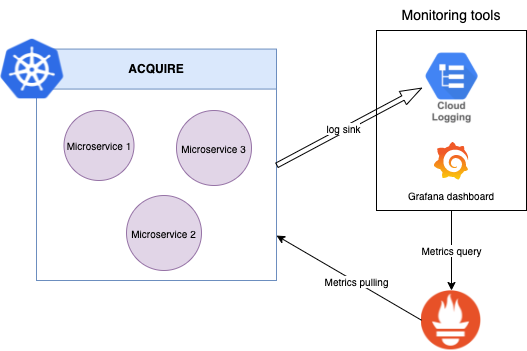
\includegraphics[scale=0.4]{src/thesis/img/background/service-monitoring.png}
    \caption{UnityAds microservices monitoring diagram}
    \label{fig:background:monitoring}
\end{figure}

This architecture is running on a Kubernetes cluster that is deployed on Google Cloud \cite{hunter2018google}. For logging, the services are using the standard Google Cloud Logging tool \cite{GoogleLogging}, which simplifies the process for the storage and exploration of them. But logging is only one of the relevant parts for monitoring, as metrics are also essential to know the overall system's health.\\

In order to collect the metrics for the different microservices of the system, Prometheus \cite{turnbull2018monitoring} is the selected tool. It works by pulling relevant metrics from microservices and infrastructure, and afterward, those metrics can be accessed using its custom query language. On top of it, some Grafana dashboards \cite{hoang2020research} can be handcrafted to visualize those metrics on time series plots. This typical setup works well as it combines the possibility of exploring error logs and even tracing the endpoint calls for the microservices on a fine granularity, using standard Google Cloud tools such as the profiler \cite{thakurratan2018google}, and at the same time presents a visual representation for the metrics of the system, such as error rate, uptime or throughput, using a time-series format.\\

\subsection{Problem definition}
\label{sec:problem-definition}

%% Describe the problem from different angles, depending on the stakeholders involved.

%% - Public APIs team: Describe that from our side the requirements is having more
%%                     visibility in the term of the errors that are generating through
%%                     our API calls from the engineering part of view.

%% - Product management: Describe that from the product side, it is important to know the high
%%                       level errors as they are in contact with the client, and they have to 
%%                       contact them in case that they are doing some wrong integrations, for example
%%                       if they hit the rate limits.

%% - Security team: From their perspective it is important to set some visibility on the high level errors
%%                  in case that some individual malicious user is doing some kind of attack to the system.

Even though the monitoring setup adopted by the Acquire unit on UnityAds works well in many cases, it has some limitations related to the monitoring of the Unity Services Gateway. First of all, it is noteworthy to say that Unity Services Gateway is another microservice, so the setup represented in figure \ref{fig:background:monitoring} is enough for metrics and architecture monitoring. Nevertheless, it has some limitations for business logic monitoring \cite{von2009decision}.\\

A gateway of a Domain-Oriented microservices architecture (DOMA) is in charge of handling some high-level responsibilities (section \ref{sec:microservices-gateway}). The main advantage of that setup, is that those tasks are shared across microservices and there is a single place where this logic is implemented and maintained. But on the other hand, the teams responsible for the microservices that are directly dependant on the gateway might want some visibility on the events generated by handling that logic.\\

To give a concrete example for this problem, let's consider only rate-limiting responsibility \cite{raghavan2007cloud}, which is vital to prevent common attacks \cite{jhaveri2012attacks} such as DDoS \cite{mirkovic2004taxonomy} or unlimited API scraping \cite{WebScrap}. The gateway's commitment corresponds to automatically rejecting the requests that had tried to access the server multiple times. To do that, it has to keep a temporal database that stores the count for how many requests the user had done on a concrete time window.\\

Considering this error type, different stakeholders would be interested in knowing more about the events associated with this error and that currently don't have that much information. The following subsections are will introduce them.

\subsubsection*{Public APIs team}

This team is responsible for developing a set of public APIs that allow advertisers to manage their advertisement campaigns programmatically. Usually, those advertisers had built custom integrations with UnityAds and want to run adverts on different platforms simultaneously to maximize the visibility of their campaigns.\\

The engineering team is contacted when some advertiser is constantly receiving errors from the APIs because it has reached the established rate limit for the endpoint they are trying to consume. This can happen for a variety of reasons, maybe they want to fetch multiple resources at the same time, or there is an error in the implementation that causes the endpoint to consume the rate limit quota. With the current setup, it is tough to trace back the reasons as even if the engineering team can access the logs, as they might not contain all the information in a convenient format.

% Another drawback is that the engineering team does not notice the problem beforehand, but only after it happens and the clients have already contacted them.

\subsubsection*{Product managers and client partners}

Product managers and client partners are the intermediaries between the engineering team and the clients that consume the APIs or any other connected service through the gateway. This is also why they want to get some visibility in which clients are hitting the rate limits on the gateway level as they can contact them directly to ensure that their integration or their usage of the company's services is correct and give assistance in that regard if needed. In that way, customer satisfaction could be improved with respect to the current status, where is the client who usually contacts if they are experiencing some errors.\\

In that sense, this team is interested in having some visual tool to access that information because accessing the logs console using a series of queries requires some previous background that those professionals might not have.

\subsubsection*{Security team}

The security team wants to know more when specific clients or users make several requests to the services. In case those calls are coming from a malicious user or a not-identified client, it could be banned for preventing any further attack \cite{jhaveri2012attacks}.

\clearpage
\section{Requirements engineering}
\label{sec:requirements-eng}

%% Taking into consideration that everyone has clear who are the stakeholders and what is the structure of the
%% company and the microservices involved, now we have to do the requirement analysis.

%% First of all, it is important to state why it is not possible to store things on Prometheus.

%% We can list the project requirements like:

%% - We need to do a clear definition of the errors that we want to log.
%% - The logging technology has to support a lot of stress as we are having x (collect the number of average requests).
%% - The provided solution has to be cloud agnostic (this is why some part has to be implemented in Terraform or using an external service).
%% - We need a visual tool in order to communicate effectively with the stakeholders.

Having presented the background necessary to understand the thesis project in Section \ref{sec:background}, this section will cover requirements engineering.\\

Requirements engineering is the process of establishing the desired requirements to be met by the project \cite{hay2003requirements}. Section \ref{sec:req-methodology} will define the methodology to be followed to gather the requirements, and Section \ref{sec:req-analysis} will analyze these requirements. Finally, Section \ref{sec:research-questions} will present the research questions that will serve as the guiding thread of this thesis.

\subsection{Requirements engineering methodology}
\label{sec:req-methodology}

Before performing the requirements analysis, it is essential to clarify which methodology will be followed to identify the project requirements. In this case, the framework proposed by David C. Hay \cite{hay2003requirements} for requirements engineering, which consists of three steps, is selected:

\begin{itemize}
    \item \textbf{Eliciting requirements}: this phase is where all the requirements will be discovered following the selected gathering methodology.
    \item \textbf{Recording requirements}: The second phase consists of the documentation of the requirements previously collected.
    \item \textbf{Analyzing requirements}: Finally, those requirements have to be analyzed in order to see if they are clear, complete, concise, and unambiguous.
\end{itemize}

For the elicitation of requirements, the selected method is stakeholders identification \cite{mitchell1997toward}, which consists of selecting individuals or groups interested in the product or function to be developed and asking them what the desired characteristics they expect from the product are. This method is the most appropriate for our project since it will only have an internal impact as external customers will not use it. The list of stakeholders for this project is given in section \ref{sec:problem-definition}.\\

To record and document the requirements expressed by the stakeholders, there were two methods: the first was to use message threads in Slack, which is the internal communication platform, where relevant stakeholders could set their expectations, and the second method was to organize some meetings, based on the framework of the Joint Requirements Development (JRD) Sessions \cite{hay2003requirements}, to discuss the project and the expected results. At these meetings, a log was drafted to keep track of the issues discussed.

\subsection{Requirements analysis}
\label{sec:req-analysis}

The last step of the chosen requirements engineering framework consists of performing an analysis of the requirements gathered from stakeholders. In that sense, the solution that is going to be presented for solving the problem stated in section \ref{sec:problem-definition} needs to meet the following requirements:

\begin{itemize}
    \item Clear definition on which are going to be the high-level responsibilities that the gateway will handle and which errors the gateway can generate associated with those.
    \item Establish a format for the generated errors. They need to store all necessary fields in order to be traced back and visualized afterward.
    \item Map possible errors and gateway responsibilities to the different endpoints that clients can consume.
    \item Select a suitable data store for the errors. Data storage needs to be easily integrated with the current cloud setup and must ensure the acceptance of a standard query language that allows the integration with third-party tools.
    \item Data ingestion has to be cloud-agnostic. This means that the error logging pipeline, from the event emission to the storage, has to be done with a technology that ensures compatibility with multiple cloud providers.
    \item Develop a visualization tool that allows stakeholders to access the errors generated at the gateway level easily.
\end{itemize}

\subsection{Research questions}
\label{sec:research-questions}

%% Taking into consideration the previous requirement analysis we can state down the research questions.

This project aims not only to satisfy the specific need for a technical feature but also to generate a set of tools and practices that can be used in the future by any other organization operating a DOMA. Therefore, this project needs an extensive investigation and planning phase, which these three research questions will guide:

\begin{itemize}
    \item[\textbf{Q1}] \textit{What is the best way to represent the possible high-level errors that a DOMA gateway can produce?}
    \item[\textbf{Q2}] \textit{What is the optimal technology for storing the errors that a DOMA gateway can produce?}
    \item[\textbf{Q3}] \textit{How to correctly visualize and communicate with the stakeholders the errors a DOMA gateway can produce?}
\end{itemize}

The objective of the thesis is to produce a series of software artifacts and standards that will satisfy the research questions and, therefore, the technical requirements of the stakeholders.

\clearpage
\section{Literature review}
\label{sec:literature-review}

%% In this section is where all the technologies used are reviewed. For sure having the following subsections:

This section aims to provide a broad review of some topics relevant to the development of this thesis. The first subsection provides a review of today's essential service architectures, including the new DOMA architecture. The second subsection provides a review of observability and monitoring issues. REWORD-THIS!!!!

\subsection{Software architectures review}

%% 5 pages
%% In this section we can include the following: (5 pages)
%% - Brief introduction about the theoretical aspects that are going to be discussed.
%% - Service Oriented Architectures (SOA)
%% - Microservces architecture.
%% - Domain oriented microservices architecture. Maybe introduce the gateway here or in another page.

Domain Oriented Microservices Architecture (DOMA) is the paradigm that many large organizations are adopting to organize their software systems and the most suitable to describe the software architecture of the Acquire unit (Section  \ref{sec:acquire-architecture}). This section offers a review of the software architectures that led to the development of DOMA.\\

Software architecture is a fundamental topic in software engineering. Its main objective is to investigate the optimal way to organize software processes and artifacts to ensure that they can function properly and communicate with each other to accomplish their tasks \cite{shadija2017towards}. According to E. Perry and L. Wolf \cite{perry1992foundations}, the term \textit{"architecture"} was introduced into software engineering in the 1980s to evoke the notions of abstraction and coding. It is still relevant today to define the layout of software systems in different enterprises.\\

One of the initial paradigms that established a breakthrough in how software systems were organized was the introduction of object-oriented programming (OOP) \cite{dahl1972chapter}, which was the first attempt to encapsulate data, offering a limited set of operations to access and modify it. It also introduced the concept of interfaces \cite{snyder1993essence}, which are the entry point that agents external to the object had to access. Although OOP established a solid foundation for creating more complex systems, it was still not sufficient to map business functionalities, which were later satisfied using more complex software paradigms. In the following subsections, those complex paradigms that are capable of mapping business functionality directly will be explained.

\subsubsection{Service-oriented architecture}

Service-Oriented Architecture (SOA) is a software paradigm that consists of packaging software systems into services that can be presented to the user in condensed packages that can be accessed through a well-defined protocol \cite{sprott2004understanding}. The rise in popularity of SOA coincides with the establishment of web protocols that allow software systems to communicate effectively.\\

The usage of those services can be done in two different ways. On the one hand, services can be consumed at run time by binding them into the code; thus, the packaging of the services is done in software libraries \cite{alahmari2010service}. On the other hand, those services can be consumed using some web protocol; in this case, some standards can be used to establish a data format, such as Web Service Description Language (WSDL) or Simple Object Access Protocol (SOAP).\\

Even though SOA is a giant step forward in the design of software systems, mainly because it helps on the scalability and reusability of components effectively, it can also present some drawbacks:

\begin{itemize}
    \item Services can contain many functionalities and a big codebase, which can be challenging to manage if the engineering team is constantly growing.
    \item If the business domain requires many functionalities that can be grouped logically in the same service, it can rapidly become a monolith. 
    \item Adding new functionalities to the system usually implies that the whole service has to be deployed simultaneously, which can be error-prone.
    \item Data storage is a central piece of software systems. It can also be the communication point between services, which can cause inconsistencies as several services might get access to the same data.
\end{itemize}

\begin{figure}[h]
    \centering
    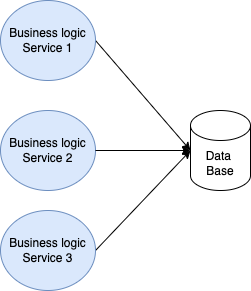
\includegraphics[scale=0.4]{src/thesis/img/literature-review/SOA.png}
    \caption{Diagram describing SOA}
    \label{fig:soa-architecture}
\end{figure}

This software architecture might be helpful in the initial stage of companies or organizations, where services are minimal and the functionalities are not entirely developed. But the pain points might arise when operating on a different scale. The initial architecture of Applifier can be considered as SOA (figure \ref{fig:background:applifier-architecture}), as it shared the same structure and had to deal with similar drawbacks.

\subsubsection{Microservices architecture}
\label{sec:microservices-architecture}

Microservices architecture is a novel approach that has gained a lot of interest both from the industrial and academic perspectives to solve the problems that traditional service architecture presents.\\

Many authors have tried to give precise definitions for microservices to establish a framework that can help both engineers and researchers develop applications that could tackle the original problems of software services.\\

One of the most relevant definitions is done by Dragoni et al. \cite{dragoni2017microservices}: \textit{"A microservice is a cohesive, independent process interacting via messages."} This definition is quite interesting because it is not centered on the size of the service, which is one of the debate points of the description due to the introduction of the word \textit{"micro"} on it. It also emphasizes the concept of independence and remote communication, one of the critical points of modern microservices, which are usually deployed independently and communicate with each other using a well-known protocol.\\

In that regard, the definition of Johannes Thönes certainly expands some relevant aspects \cite{thones2015microservices}: \textit{"Microservice is a small application that can be deployed independently, scaled independently, and tested independently, and that has a single responsibility."} One of the emphasis points on this definition is the independence on the deployment and testing, which is one of the key advantages that make microservices useful when managed by a growing team of engineers. Apart from that, Thrones points out the single responsibility principle that should always be kept in mind when designing microservices.\\

Following the classification of Lewis et al. \cite{MicroservicesCharacteristics} microservices should share the following characteristics:

\begin{itemize}
    \item \textbf{The modularity of services}. As in SOA, microservices offer a modular functionality that can be reused easily. The main difference between both is that microservices could be deployed independently, whereas, on SOA, each release implies a complete deployment of the service.
    \item \textbf{Organised around business capability}. On traditional software systems, teams are organized into different functional areas; for example, one group would be responsible for engineering one service and another for deployment and testing. In that schema, if there is a failing deployment, the responsibility is shared across the teams, which can cause some delays as the issue can not be handled within an organizational unit.
    \item \textbf{They are product not projects}. In SOA, each service is mapped into a business requirement; on the contrary, on microservices, one business requirement aims to be mapped to multiple microservices to reduce the amount of responsibilities of each one.
    \item \textbf{There are intelligent endpoints and dumb pipes}: The main logic has to be placed on the microservices that are accessed via endpoints. There have to be few communication middlewares (pipes) with actual logic.
    \item \textbf{Decentralized data management and governance}: One of the main characteristics of microservices is that data is no longer the common point between services because each microservice has its independent data store.
\end{itemize}

\begin{figure}[h]
    \centering
    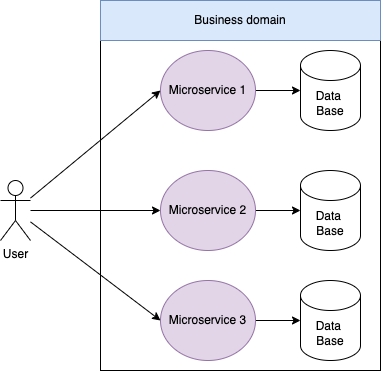
\includegraphics[scale=0.4]{src/thesis/img/literature-review/microservices.png}
    \caption{Diagram describing microservices architecture}
    \label{fig:microservices-architecture}
\end{figure}

Microservices represent a giant step forward in developing software architectures, as they present many \textit{operational} benefits compared to SOA. Nevertheless, they are not a silver bullet as they also introduces some significant drawbacks, such as:

\begin{itemize}
    \item The introduction of performance issues. The remote procedure calls (RPC) used between microservices to communicate can introduce some delays as they have to be resolved over the network.
    \item Problems on the data aggregation.  As microservices remove a shared data storage in favor of a decoupled data governance if some complex data has to be retrieved that involves some integration between different sources.
    \item Difficulties in introducing new features. In a microservice architecture, introducing a new feature might involve changing several services, which can delay communication, validation, and code review.
\end{itemize}

\subsubsection{Domain-oriented microservices architecture}
\label{sec:domain-oriented-microservices-architecture}

% The schema on this part has to be as it follows.
% - Introducing the main problems that microservices architecture present for large scale companies.
% - The different parts of the microservices architecture: domains, layers and gateways.
% - Review of Unity´s initial DOMA architecture.

The latest revised architecture will be DOMA, presented by Gluck A. in 2020, on behalf of Uber's engineering team \cite{DOMAUber}. The primary goal of DOMA is to mitigate the problems that microservices architecture presents in large enterprises that have hundreds of interconnected microservices.\\

In these companies, there are some additional problems to those discussed in section \ref{sec:microservices-architecture}:

\begin{itemize}
    \item Knowledge sharing and architecture onboarding. When the number of microservices is significant, the understanding of the system becomes complex. That increases the onboarding time for new engineers, which causes an operational cost for the company.
    \item Difficulties to to debug and identify a problem. When considering hundreds of interconnected services, if a call in any of them introduces some delay or bug, engineers have to trace back the call stack, requiring substantial cross-team effort.
\end{itemize}

DOMA is a new software design pattern iteration that tries to tackle these problems. The main principles are extracted from Domain-Driven Design, a paradigm introduced by E. Evans and EJ. Evans \cite{evans2004domain}, which defines software design based on the domain or business-specific needs. In that regard, DOMA is the direct application of Domain-Driven design to microservices design in an extensive network of distributed and interconnected services.\\

\begin{figure}[h!]
    \centering
    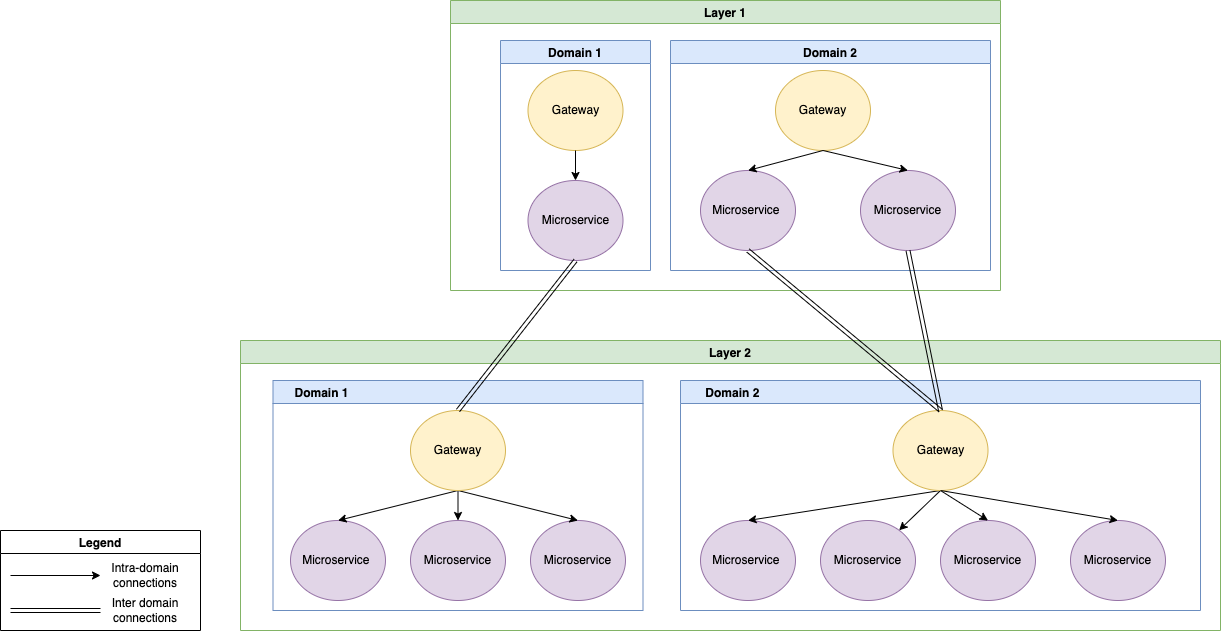
\includegraphics[scale=0.3]{src/thesis/img/literature-review/doma.png}
    \caption{DOMA architecture diagram, with representation of the two communication types}
    \label{fig:my_label}
\end{figure}

DOMA is adopted on organizations as an iteration of a pre-existent microservices software architecture. Four main elements have to be introduced \cite{DOMAUber}, to do that transition:

\begin{itemize}
    \item \textbf{Domains}: A domain is a collection of related microservices. The main design challenge of this element is to decide how big the domain should be and how many microservices should contain.
    \item \textbf{Layers}: A layer is a collection of domains. The primary behavioral change is that we can consider that the layers are grouped into a stack, where the layer defines the dependencies between the domains that they belong to in the pyramid.
    \item \textbf{Gateway}: The gateway is the single point of access of each domain. It is the public interface of the domain, and it should prevent access to individual services and implement several high-level responsibilities.
    \item \textbf{Extension architecture}: the extension mechanism is a procedure for adding extra functionalities. This is important to respect the open-closed principle of the domain. It is remarkable to state that this can not be achieved on all domains as it depends on the nature of the handled data.
\end{itemize}

The introduction of DOMA is recent, so there is not much research on how to populate those four elements with concrete business requirements to transition a microservices architecture into a successful DOMA. The only available public example is offered in the article by Uber Engineering \cite{DOMAUber}, where they provide an interesting view on how to distribute the layers pyramidally, where the base of the pyramid represents broad functionalities that can be used across the organization, such as storage or networking services. In contrast, concrete client-facing functionalities are at the top of the pyramid. This interesting approach guarantees that the layers are isolated, and dependencies flow from top to bottom.

\subsection{Microservices gateway}
\label{sec:microservices-gateway}

This section is intended to extend the knowledge presented in the previous section about microservices gateways. As stated before, gateways are an essential element in DOMA, and their primary purpose is to isolate the domains of microservices and work as the single entry point. Even though they represent a crucial element in DOMA, they can also be used in a simple microservices architecture.\\

\begin{figure}[h!]
    \centering
    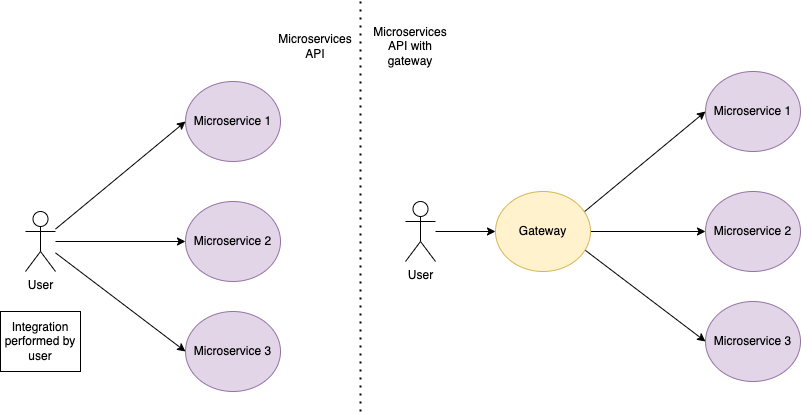
\includegraphics[scale=0.3]{src/thesis/img/literature-review/gateway.png}
    \caption{Diagram comparing the call of a microservice architecture with or without gateway}
\end{figure}

On Microservices Patterns, by C. Richardson \cite{richardson2018microservices}, several reasons why creating an API gateway is vital on a microservices architecture are introduced.

\begin{itemize}
    \item Each microservice exposes a minimal set of fine-grain API endpoints. To compose a more meaningful and high-level API call, the information of many microservices has to be integrated somehow. That responsibility should ideally not lie on the consumers of the services.
    \item The users do not need to know the internal details of microservices architecture to respect the company's privacy and internal structure. Due to this, they rather interact with some proxy instead of calling the specific microservices.
    \item The communication protocols between microservices can be very diverse. Clients would prefer only to use one communication protocol to request resources on the systems rather than preparing their custom data integration.
    \item Several high-level responsibilities are shared between microservices, and they would be better managed on a central point rather than re-implementing the logic for each service.
\end{itemize}

Each point of this list defines a valid reason for considering the creation of a microservices architecture gateway; nevertheless, the last one is the most relevant for this thesis and is the one that will be explored in-depth.\\

As this thesis aims to monitor the high-level errors of a microservices architecture gateway, it is necessary first to define the responsibilities it has to take. The high-level responsibilities stated by M. Thangavelu et al. \cite{UberGateway} will be considered for this definition.

\begin{itemize}
    \item \textbf{Auditing pipeline}. maintaining a registry of all the access and operations that the gateway performs. This thesis aims to improve the logging when referring to the error generated by the stated responsibilities.
    \item \textbf{Identity}. Each access to the service has to be authenticated and authorized, and that responsibility should lie on a central software piece like the gateway.
    \item \textbf{Rate limiting}. That refers to the capacity of the system to prevent malicious attacks caused by an uncontrolled number of recurrent requests.
    \item \textbf{Documentation}. Ideally, all API calls should be documented on a central repository with a standard format.
    \item \textbf{Response fields trimming}. As the gateway works as a proxy for the backend microservices, it would be helpful to have the possibility to specify the omission of specific fields on the user's responses.
    \item \textbf{Datacenter affinity}. There can be some logic on the gateway that could redirect user calls to certain physical regions where the data can be retrieved faster.
    \item \textbf{Short-term user bans}. Temporarily banning users who had malicious behavior on the system can be one of the solutions to deal with cyber-attacks. That responsibility should be delegated to a central software piece rather than be shared across the microservices.
\end{itemize}

Considering those high-level responsibilities, in section \ref{sec:gateway-configuration-file} the errors related to each of them will be defined.

\subsection{Open-source microservices gateways}
\label{sec:industry-gateways}

This section will explain two of the main industry-relevant microservices architectures gateways that are open-sourced and can be incorporated into any company's current architecture. The main idea is to simplify the development of a gateway, having all the benefits already explained in section \ref{sec:microservices-gateway}, while also reducing time-to-market as the primary development effort can be centered on creating the end-product. The two gateways that will be relevant for this analysis are Kong and Zuul, both open-source solutions.

\begin{itemize}
    \item \textbf{Kong Gateway}: Kong is the most popular open-source microservices gateway nowadays \cite{KongGateway}. It is a containerized Lua application that can be extensible by custom plugins and executed within a Kubernetes deployment. Its main advantage is that it is fully configurable, so the different high-level responsibilities can be configured depending on the protocol or technology that is preferable to use.
    \item \textbf{Zuul Gateway}: The Netflix engineering team created Zuul gateway as part of their internal stack and then released it as open-source in 2018 \cite{ZuulGateway}. Its main characteristic is that it is built for resisting a high volume of queries. It is the central entry point for all the cloud infrastructure at Netflix, having more than a million requests per second. The architecture of it works in layers. First of all, there is a module that sets all the correspondent network settings and connection protocols, and then there are different filters that are used for decorating the requests before being forwarded to the backends.
\end{itemize}

As it can be seen, both options offer a solution for companies that operate on a big scale and that have a considerable volume of traffic. In section \ref{sec:gateways-comparison}, those solutions will be examined in depth to be compared with the proposed solution in this project's scope.

\subsection{Observability and Monitoring}
\label{sec:observability-monitoring}

%% In this section we can differentiate the following topics: (3 pages)
%% - Observability and Monitoring definition.
%% - Application of observability and monitoring to microservices.
%% - Data observability.
%% - The four pillars of data observability (check one of the articles).

% Introduction to monitoring and observability
% Which is the state of the art on it and offer a plot with the authors.
%

Observability and monitoring are hot topics in software system maintenance, and it is especially relevant to review them applied to microservices architecture \cite{ObservabilityvsMonitoring}. Hence, the objective of this section is to give a theoretical introduction to both topics, a review of the current \textit{state-of-the-art}.\\

It is common to confuse both observability and monitoring as their objective is to check whether something in the system is not working as it should \cite{ObservabilityvsMonitoring}. Nevertheless, monitoring is based on taking metrics of quantifiable elements such as CPU usage, memory usage, or network traffic \cite{MonitoringIEEE}. The basic procedure for monitoring any system is by querying it directly to obtain those metrics and set up visual dashboards and alerts that will warn if the behavior is not the expected. This method is quite effective for maintaining traditional monolithic applications' health as the resources they consume are centralized, contrary to microservices or DOMA, where they are distributed over a network. Also, monitoring presents a clear disadvantage as the problems are usually identified when the metrics' values show a higher value than a certain threshold, which might be too late to react to an incident.\\

On the other hand, observability is similar on purpose but different on methodology. Rudolph E. Kalman introduced the term observability in 1960 on the control systems field \cite{kalman1960general}. The basic definition is: \textit{"Observability is a measure of the wellness of the internal state of a system inferred from the knowledge of its external outputs."} Even if it was first invented for the control systems field, observability has been applied to modern software architectures, such as microservices. Attending to that classic definition, the inference of the internal state had to be done by producing a set of outputs from the highly-observable software service that it is being maintained, and that is done by generating a set of logs and traces \cite{picoreti2018multilevel}.\\

In that regard, to investigate \textbf{Q1} and generate a valuable solution, it is needed to create an observability + monitoring tool. The observability side of the project will be responsible for the generation of logs that will contain enough information about the internal state and the high-level errors that the gateway handled. On top of it, a monitoring platform had to be created to visualize those responsibilities graphically, hence addressing \textbf{Q3}.\\

It is also relevant to review the previous studies in the field of services monitoring. To narrow the scope of the research, only previous studies centered on microservices are considered. Furthermore, only the ones provide a novel approach to bridge the gap between the complexity of distributed microservices architecture and its monitoring \cite{niedermaier2019observability}.\\

First of all, Yang et al. \cite{yang2018transparently} propose a new approach for capturing the request execution path (REP) transparently. This novel method categorizes the events generated at a microservice level, and the relationships between those events are identified to construct a monitoring tool that could effectively trace the REP. The way this study categorizes the events is similar to the work done for the categorization of the DOMA Gateway events done for this thesis (Section \ref{sec:gateway-configuration-file}).\\

Sun et al. \cite{sun2018constraint} presented an analysis of many microservices architectures on the complexity analysis topic, pointing out that they do not provide any valuable information about their internal state. Hence, the observability procedures were not working correctly, and some improvements have to be made.\\

Jongh et al.\cite{johng2018estimating} formulate a different study where benchmarking and simulation are used on a combined approach in order to monitor execution times. This study is centered on monitoring execution performance, offering a concrete technical solution instead of concrete surveys and definitions.\\

In that regard, Lin et al. \cite{lin2018microscope} present a study whose aim is to propose a new method for root cause detection, where the errors are identified using causal graphs. This work focuses on identifying and monitoring the errors caused in distributed systems and how they are propagated across the architecture.\\

Finally, Gupta et al. \cite{gupta2018runtime} proposed a new way for monitoring continuous deployment on rapidly changing companies (with the independence of the size of the product). On that approach, data mining techniques are applied to the logs of highly-observable microservices to discover the differences between deployed versions on microservices.\\

\clearpage
\section{Technical solution}
\label{sec:technical-solution}

%% The outcome of this thesis are 3 technical solutions.

This section will cover the technical solution developed on the scope of this thesis. The first subsection will introduce the gateway configuration file, the contract used to match the endpoints that the gateway exposes with the high-level responsibilities it will address. The second subsection will explain the error definition format and the data pipeline implemented to store the errors generated at the gateway level. Finally, the third subsection will introduce the visualization dashboard for the gateway errors.

\subsection{Gateway configuration file}
\label{sec:gateway-configuration-file}

After having discussed the high-level responsibilities that the gateway of a DOMA should have (section \ref{sec:microservices-gateway}), in this chapter, one of the main outputs obtained from this thesis is introduced, which is the definition of a route-level configuration format for the gateway in order to solve \textbf{Q1}.\\

A route-level configuration format is a standard that can be used to state down all the resources that the gateway of the domain exposes to the public and the associated responsibilities attached to each route. Having this standard defined will have many significant advantages, such as:

\begin{itemize}
    \item It can be used as the primary source of truth of the resources that the gateway exposes.
    \item The generation of the endpoint's documentation can be automatized; therefore, all the teams involved in the microservices do not need to do it by themselves.
    \item This standard defines a contract on what the endpoint handlers should do when managing the responsibilities. The engineers that are going to implement the proxy should fulfill the specifications of the standards, and the endpoints consumer should rely on those responsibilities.
    \item There are some literature examples of composable gateway logic \cite{UberGateway}; this standard can be the starting point of this automated gateway generator. 
\end{itemize}

In the following subsections, there is going to be an explanation of the general structure of this configuration file, using YAML as the format, as well as each filter that can be specified to fulfill each gateway's responsibilities (section \ref{sec:microservices-gateway}).

\subsubsection*{General structure}

The general structure of the configuration file is as follows: \\

\clearpage

\begin{lstlisting}[language=json,firstnumber=1]
- path: path/to/my/resource
  envs: ['prd', 'stg', ... ]
  methods: ['get', 'post', 'put' ... ]
  endpointFilters:
    ...
  transport: 'http'
\end{lstlisting}

There is one entry per resource on the gateway configuration file, and the following elements will specify each entry:

\begin{itemize}
    \item \texttt{path}: This is the URL that will be used to do the operation on the system, and it is also the identifier of the resource.
    \item \texttt{env}: The environment where the gateway is executed. Usually, there are three different environments considered in software engineering: local, staging, and production.
    \item \texttt{methods}: The HTTP method to be used: put, post, get, patch... those method corresponds to CRUD operations \cite{martin1983managing}.
    \item \texttt{endpointFilters}: Those filters are the responsibilities that the gateway will take. They are going to be defined in the following subsections.
    \item \texttt{transport}: The transport method used. Usually, it will correspond to HTTP, but other protocols like NATS can be specified.
\end{itemize}

\subsubsection*{Auditing filter}

The first filter specified, which is going to be contained under the \texttt{endpointFilters} specification, is going to be the filter used for the auditing responsibility of the gateway. The structure is as follows:\\

\begin{lstlisting}[language=json,firstnumber=1]
  endpointFilters:
    - auditing: boolean
\end{lstlisting}

To keep this filter simple, there will be only a boolean flag that will determine if there has to be any kind of logging or auditing at the gateway level for the specified endpoint.

\subsubsection*{Identity filter}

This filter specifies if there has to be any authentication or authorization for consuming the endpoint resources. The structure of the filter is:\\

\begin{lstlisting}[language=json,firstnumber=1]
  endpointFilters:
    - authentication: service-account | OAuth
    - authorization:
	    create: permission-identifier
	    read: permission-identifier
	    update: permission-identifier
	    delete: permission-identifier
\end{lstlisting}

First of all, the authentication section specifies how the user has to be identified on the system. In this example, two options are shown: service accounts and OAuth \cite{OAuth2}, but there can be many other methods and should be specified by the systems designers.\\

On the authorization side, the consideration has been to use Role-Based Access Control (RBAC) \cite{ferraiolo2003role}, which assigns one role to each user and specifies a set of permissions for each role. The specific CRUD operation can only be performed if the permission matches the one resolved for the user who tries to consume the resource.

\subsubsection*{Rate limiting filter}

Rate limiting filter defines the number of access that the gateway will accept on a certain period of time. The structure of the filter is the following: \\

\begin{lstlisting}[language=json,firstnumber=1]
  endpointFilters:
    - httpMethods: [get, put, patch, delete] // http methods to limit
    - perSecond: {prd: 6, stg: 100, local: 10000}
    - perThirtyMinutes: 4000
\end{lstlisting}

There are three fields that the filter accepts; the first one is the HTTP methods that are considered for the rate-limiting, the second is the number of accesses that the gateway accepts in one second, and the third one is the number of access that it accepts in thirty minutes. For the last two properties, it can be specified the number of accesses or an object with three properties referring to the three possible environments and a number for the rate-limiting on those.

\subsubsection*{Documentation filter}

This simple filter specifies if any documentation for the endpoint at the gateway level has to be produced. There might be private endpoints where the consumption is done only within the organization, so creating external documentation might not be desired. The structure of it is as follows:\\

\begin{lstlisting}[language=json,firstnumber=1]
  endpointFilters:
    - documentation: boolean
\end{lstlisting}

\subsubsection*{Response fields trimming}

As the gateway should work as the proxy for all the microservices under a domain, we may want some fields not exposed outside of it, which is the purpose of the response field trimming. The structure is as follows:\\

\begin{lstlisting}[language=json,firstnumber=1]
  endpointFilters:
    - responseTrimming: [field1, field2, ...]
\end{lstlisting}

The fields that are included in the array are not going to be forwarded to the endpoint consumers.

%% In this section describe the different high level errors and the standard that we are defining for them.
%% Check out the ones defined previously by Uber gateway API.

\subsection{Events collection and storage}

%% The things that need to be covered here are:

%% - Planning (Using AirTable and estimation)
%% - Implementation on the gateway side. Explain that Unity currently has a logging tool enabled and we only had to log certain events gathering the requests.
%% - Terraform implementation. This part is where it can be explained how we use terraform and how to the problem cloud-agnostic.
%% - BigQuery setup.

As stated in section \ref{sec:req-analysis}, one of the requirements for this project is to create a tool that stores and visualizes the high-level errors that the gateway is generating. This section covers the development of that tool, explaining the definition of the error format, the creation of the events gathering, the data pipeline for storing those events and finally the selection and setup of the data storage technology.

\subsubsection{Error event definition}
\label{sec:error-event-definition}

This subsection covers the definition of the error events that will be collected on the data storage to be visualized in the future. The main objective of this is that it should share many standard fields that can be used to identify the error for all the gateway high-level responsibilities (section \ref{sec:microservices-gateway}).\\

For doing that, the approach consists of having some general fields independent of the error event generated, which will be used to locate the endpoint that was called and that caused the error. Apart from that, some specific fields will be stored depending on the high-level responsibility that caused the error, and the purpose for this is to create meaningful visualizations afterward. It is essential to state that only the rate-limiting responsibility was considered for the initial implementation as it is the most important for the stakeholders. Nevertheless, it can be extended in the future as many fields can be added easily to the events.\\

The procedure for defining which are the meaningful fields that had to be stored was by presenting an RFC (Requests for comments) \cite{reynolds1987request} internally on the gateway development team, so all the people involved on it could freely give comments and ideas. As the company is using Slack as the communication platform, the RFC was shared in a Slack thread. The number of people present on the slack channel was 294 when the RFC was published, and there were 139 replies to it from people from different teams, such as project managers and engineers.\\

After that internal discussion, the agreed set of fields that the events should contain are the following ones:

\begin{itemize}
    \item \texttt{source}: It is the type of event that will be stored. They should match the gateway responsibilities (section \ref{sec:microservices-gateway}), but as stated before, as only the rate-limiting responsibility is considered for this implementation, the only possible value is \texttt{RATE\_LIMIT}. Some other values like \texttt{AUTHENTICATION} or \texttt{AUTHORIZATION} can be added in the future.
    \item \texttt{requestId}: This maps the request to a unique id that can be used to trace it back on the microservices calls. The gateway defines this unique id.
    \item \texttt{path}: The completed path of the resource requested on the query. In the context of the Unity public API an example of it can be: \\ \texttt{/advertise/v1/organizations/:organizationId/apps/:appId}.
    \item \texttt{organizationId}: It is the organization id extracted from the request's path. If that parameter is not present on the path, the value is \texttt{null}.
    \item \texttt{httpMethod}: This value is the HTTP method used in the request. This parameter is essential for distinguishing between different endpoints.
    \item \texttt{apiVersion}: As REST APIs are frequently versioned \cite{varga2016versioning}, this parameter aims to contain the different versions of the API. It is also extracted from the path, so it has a null value if it is not present on it.
    \item \texttt{apiType}: This parameter distinguishes between the two types of API endpoints, \texttt{private} and \texttt{public} ones. Private endpoints are used only internally, whereas public endpoints can be consumed by any external client.
    \item \texttt{apiNamespace}: In the context of the company, there are different types of APIs: monetization, advertising, cloud game..., and those categories are considered namespaces. This field represents the identifier of the namespace.
    \item \texttt{timestamp}: Timestamp on Unix standard time for when the event was triggered.
\end{itemize}

Apart from the previous fields, which are the common ones and shared across different errors, there is also the definition of specific fields about the rate limit responsibility:

\begin{itemize}
    \item \texttt{rateLimitReason}: this is why the rate-limiting was activated and which of the two maximum rates was reached. It can be either \texttt{tooManyRequestPerSecond} or \texttt{tooManyRequestsPerThirtyMinutes}.
    \item \texttt{quota}: Number of requests that made the rate limit reach the maximum amount.
    \item \texttt{group}: Rate limiters can be grouped to be shared across different endpoints. For that, the parser of the gateway responsibilities file (section \ref{sec:gateway-configuration-file}) had to be able to apply shared rate-limiting responsibilities to other endpoints. This field stores the identifier of the rate limiter that was hit. In case it is not present, it should have a \texttt{null} value.
\end{itemize}

After having defined the data structure for the events, the following sections will cover its technical implementation, from the collection of the event on the gateway side to the actual storage on the databases.

\subsubsection{Project planning}

Before diving into the project's technical implementation, it is relevant to give a brief overview of the project planning. To develop the project, we used scrum as the agile methodology \cite{schwaber1997scrum}, dividing the tasks into specific user stories and tasks that were executed on different sprints. The tool used for the project planning was AirTable, which primary usage was to introduce the three stories that configure the project and give an estimation based on the workforce that will execute it.\\

\begin{figure}[h!]
    \centering
    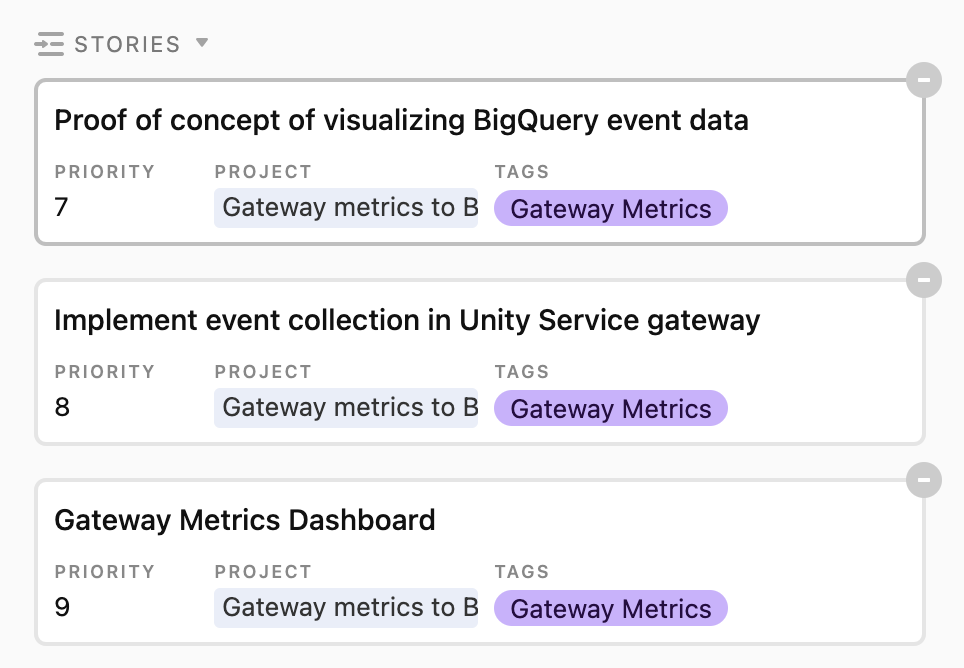
\includegraphics[scale=0.3]{src/thesis/img/technical-solution/project-planning.png}
    \caption{Project planning on AirTable}
\end{figure}

The three project stories that configured the project were:

\begin{itemize}
    \item \textbf{Proof of concept of visualizing event data}: As we were unsure how to use the selected technologies for development, first, it was needed to build a proof of concept with dummy data to configure all involved parts. Also, this story included the publishing of the RFC for the event structure described in section \ref{sec:error-event-definition}.
    \item \textbf{Implement event collection in Unity Services Gateway}: This story includes the implementation of the events collection on Unity Services Gateway as well as the setup of the data pipelines, described in section \ref{sec:event-gathering} and \ref{sec:log-sink} respectively.
    \item \textbf{Gateway metrics dashboard}: This story covers the implementation of the custom plots used on the visualization step; this is explained in more detail in section \ref{sec:visualization-dashboard}.
\end{itemize}

To fulfill the three stories that composed the project, the total execution time was one month, which was close to the estimated time, only differing on a couple of days.

\subsubsection{Data storage technology selection}

This section aims to explain why a particular storage technology is selected for storing the generated gateway errors, thus answering \textbf{Q2}. To define the optimal storage technology, three criteria have been considered.

\begin{itemize}
    \item[\textbf{C1}] \textbf{price}: The monthly price that the organization has to spend on the selected technology.
    \item[\textbf{C2}] \textbf{Data access}: This criterion sets how easy it is to consult the data stored using an standard query language such as SQL.
    \item[\textbf{C3}] \textbf{Integration with the current cloud setup}: most modern organizations, especially those that are big enough to deal with a gateway for a microservices architecture, are operating using a cloud provider. In that sense, this criterion sets the easiness for integrating the storage technology with the current cloud provider.
\end{itemize}

The answers for this questions might differ depending on different organizations, but should be enough for deciding the best choice among the considered technologies. For the scope of this project and considering the events generated on the Unity Services Gateway, there are three storing technologies considered in the comparison:

\begin{itemize}
    \item \textbf{BigQuery} \cite{BigQuery}: This is a data warehouse designed by Google to store, efficiently access, and analyze enormous amounts of data. One of its most interesting characteristics is that it allows access to that data using standard SQL statements.
    \item \textbf{Amplitude} \cite{Amplitude}: This is a tool used to store events produced on applications and analyze them. It is more common to use it in front-end applications to analyze user behavior.
    \item \textbf{PostgresSQL} \cite{PostgreSQL}: PostgreSQL is an open-source relational database. It has to be used on an instance in the cloud provider of our choice.
\end{itemize}

After having defined those three options, they will be compared using the three criteria on separate sections, and finally, the results will be shown in table \ref{tab:data-souces}.

\subsubsection*{C1 - Price}

It is essential to set some common values needed to compare different technologies' prices.

\begin{itemize}
    \item \textbf{Requests per month} ($N$): It is considered that 50.000 events per month is the upper bound for the number of events for all endpoints.
    \item \textbf{Size of the insertion request (KB)} ($w_i$): Another consideration is that the upper bound for insertion is 100KB per event.
    \item \textbf{Maximum size per retrieve request (MB)}: One consideration is that there can be fetched 1000 records at most when retrieving the information. This limit is set as it is the limit of Grafana, the visualization platform.
    \item \textbf{Storage per year}: Considering the number of monthly requests and the size of each new record, the storage that we will consume is around 50GB per year.
\end{itemize}

After having those variables settled, the cost calculations are going to be done for the three different storage technologies considered.

\subsubsection*{BigQuery}

First of all, the costs for BigQuery are going to be calculated based on the official documentation for the tool \cite{BigQueryDocsPricing} and on the article by Welch Al \cite{BigQueryCosts}. On BigQuery, there are three different types of costs: storage costs, query costs, and insertion costs.\\

First, storage costs are going to be calculated. Storage costs are different depending on active storage (\$0.02/GB/month) and long-term storage (\$0.01/GB/month). The consideration of a record as active or long-term is decided by Google and depends on the last time accessing it. The calculation is that 15GB would be active storage, and there would be another additional 35GB as long-term storage.

\begin{equation}
\begin{split}
    C_{storage} = \$0.02 \cdot S_{active} + \$0.01 \cdot s_{long-term} \\
    C_{storage} = \$0.02 \cdot 15GB + \$0.01 \cdot 35GB \\
    C_{storage} = \$ 0.65 / month
\end{split}
\end{equation}

Secondly, the query costs are going to be estimated. Those costs are calculated per terabyte processed (\$5 / TB), so the estimation has to be in that unit. The three variables involved in that calculation are the following:

\begin{itemize}
    \item \textbf{The number of users per day} ($n$): The estimation is that 20 will be the upper bound for daily users, as it is an internal tool that is usually not consulted every day. Considering that they access five times, the total will be around 100 estimated daily individual accesses.
    \item \textbf{The number of queries per user} ($q$): The estimated number of queries is 25 for the initial implementation of the visualization tool.
    \item \textbf{Average data usage} ($d$): The data usage is the number of max records fetched per query. This number was set before to 1000 records, so the calculation in TB is the following: $100KB \cdot 1000 = 100000KB = 1e^{-4}TB$
    
\end{itemize}

\begin{equation}
\begin{split}
    C_{query} = \$5 \cdot (n \cdot q \cdot d \cdot 30) \\
    C_{query} = \$5 \cdot (20 \cdot 25 \cdot 1e^{-4}TB \cdot 30)\\
    C_{query} = \$7.5 / month
\end{split}
\end{equation}

Finally, the last type of cost being addressed is the insertion cost. This one is the easiest to calculate, as it only consists of \$0.01 per 200MB inserted. So the total insertion cost will be:

\begin{equation}
\begin{split}
    C_{insertion} = \frac{\$0.01}{200MB} \cdot N \cdot w_i \\
    C_{insertion} = \frac{\$0.01}{200MB} \cdot 50.000 \cdot 0.1MB \\
    C_{insertion} = \$0.25 / month
\end{split}
\end{equation}

Considering those three costs, the total monthly cost ($C_{total}$) for BigQuery is estimated as it follows:

\begin{equation}
\begin{split}
    C_{total} = C_{insertion} + C_{query} + C_{storage}\\
    C_{insertion} = \$0.25 + \$7.5 +\$0.65\\
    C_{insertion} = \$8.4 / month
\end{split}
\end{equation}

As it can be seen the total monthly cost for this technology is of \$8.4 / month.

\subsubsection*{Amplitude}

Amplitude's costs are divided into three categories: starter, growth, and Enterprise. On the starter version, they offer the storage and processing of 10 million monthly events, which is more than enough for covering the expected 50.0000 monthly actions. The price for this version is free, so as it can be seen Amplitude is a good option cost-wise.

\subsubsection*{PostgresSQL}

Here the costs are not dependent on the technology itself, as PostgresSQL is an open-source database technology, but on the expenses related to the cloud provider, which in the case for this project is Google Cloud. To calculate the costs, the official documentation for CloudSQL \cite{PostgreSQLonGCP} is considered.\\

In this case, the are three variables to decide that will determine the costs, which are also dependent on the zone. In this case, we are considering London (Europe west-2) for the cost calculation in order to cover European clients:

\begin{itemize}
    \item \textbf{Number of CPUs}: It is the number of virtual CPUs allocated for processing the events, the insertions, and the queries. As the application is not customer-facing, the estimation is that only 2 CPUs will be enough. The price for each CPU is \$27.13 per month.
    \item \textbf{Memory}: The amount of memory allocated for the processing. The estimation is to have 8GBs assigned. The price is \$6.13 per GB per month.
    \item \textbf{Storage}: For the storage, same numbers as for the BigQuery section it is considered. The price is \$0.176 per GB on SSD storage and \$0.09 per GB on HDD storage.
\end{itemize}

Once those variables had been established, the total cost for this technology will be:

\begin{equation}
\begin{split}
    C_{total} = C_{CPU} + C_{memory} + C_{storage}\\
    C_{total} = \$27.13 \cdot 2 + \$6.13 \cdot 8 + \$0.176 \cdot 15 + \$0.09 \cdot 35\\
    C_{total} = \$54.26 + \$49.04 + \$5.79
    C_{total} = \$109.9 / month
\end{split}
\end{equation}

\subsubsection*{C2 - Data access}

The second criterion considered is the tool's easiness for accessing data, especially if we consider using a standard query language such as SQL. In that regard, the characteristics for each datasource are:
\begin{itemize}
    \item \textbf{BigQuery}: One of the main characteristics of BigQuery is that even though it is a data warehouse, standard SQL can be used for accessing the data on it, so that makes it convenient.
    \item \textbf{Amplitude}: One of the weak points of this tool is that the data can only be accessed via their application using click-ops, which makes the integration with external tools difficult.
    \item \textbf{PostgresSQL}: As it is a traditional relational database, it can be accessed using standard SQL.
\end{itemize}

\subsubsection*{C3 - integration with the current cloud setup}

This third criterion refers to the tool's capacity to be used in integration with the current cloud setup for its purpose. The comparison between them is as follows:

\begin{itemize}
    \item \textbf{BigQuery}: In the case of using Google Cloud Platform, BigQuery is integrated into the environment out of the box. Nevertheless, if the company already uses another cloud platform, BigQuery is not a suitable option.
    \item \textbf{Amplitude}: As it is an external platform, it can be easily used with any cloud provider to store and analyze events. 
    \item \textbf{PostgresSQL}: All modern cloud providers provide access to a database instance, so it should be effortless to integrate with any of them. 
\end{itemize}

\subsubsection*{Data storage selection based on the criteria}

Based on the three criteria, table \ref{tab:data-souces} contains a summary of the comparison between the three technologies. Based on this table and for the particular case of the Unity Services Gateway, the team decided to continue the project with BigQuery. The main factor for making that decision was that it is already integrated into the cloud environment, and it is already being used in other parts of the technical stack.\\

\begin{table}[h!]
\centering
\begin{tabular}{|l|c|c|c|}
\hline
           & C1 - Price    & C2 - Data Access & C3 - Integration \\ \hline\hline
BigQuery   & \$8.4/month   & Easy             & High             \\
Amplitude  & Free          & Medium           & Medium           \\
PostgreSQL & \$109.9/month & Medium           & High             \\ \hline 
\end{tabular}
\caption{Comparison between different data storage and data analysis technologies}
\label{tab:data-souces}
\end{table}

For the particular case of any other company trying to accommodate this solution for their specific case, it is vital to do an analysis depending on the business conditions and then decide accordingly using those three criteria.

\subsubsection{BigQuery setup}

Once it was decided that BigQuery was the technology to go with this project, the next step was to create the table containing the data and configuration. This can be easily done using the Google Cloud Console on the BigQuery section.\\

First of all, the database has to be created under the target project on Google cloud. In our case, it is the \texttt{unity-services-foundation-stg} project for staging deployment and \texttt{unity-services-foundation-prd} for production deployment (figure \ref{fig:bigquery-creation}). In this case, two databases will be created with the exact schema both for staging and production to have a separated development environment from production.

\begin{figure}[h!]
    \centering
    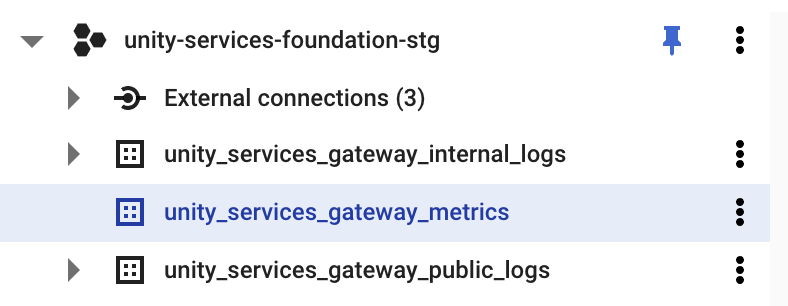
\includegraphics[scale=0.3]{src/thesis/img/technical-solution/table-creation.png}
    \caption{Table creation on staging project, exactly the same setup is reproduced on production}
    \label{fig:bigquery-creation}
\end{figure}

The schema of those databases will follow the events structure already explained in section \ref{sec:error-event-definition}. As can be seen on figure \ref{fig:bigquery-schema}, most of the variables are set to string as data type except for the required timestamp, used for data partitioning. It is also noticeable that all the columns set to \texttt{REQUIRED} on the database correspond to the common fields on the events previously explained in section \ref{sec:error-event-definition}. \\

\begin{figure}[h!]
    \centering
    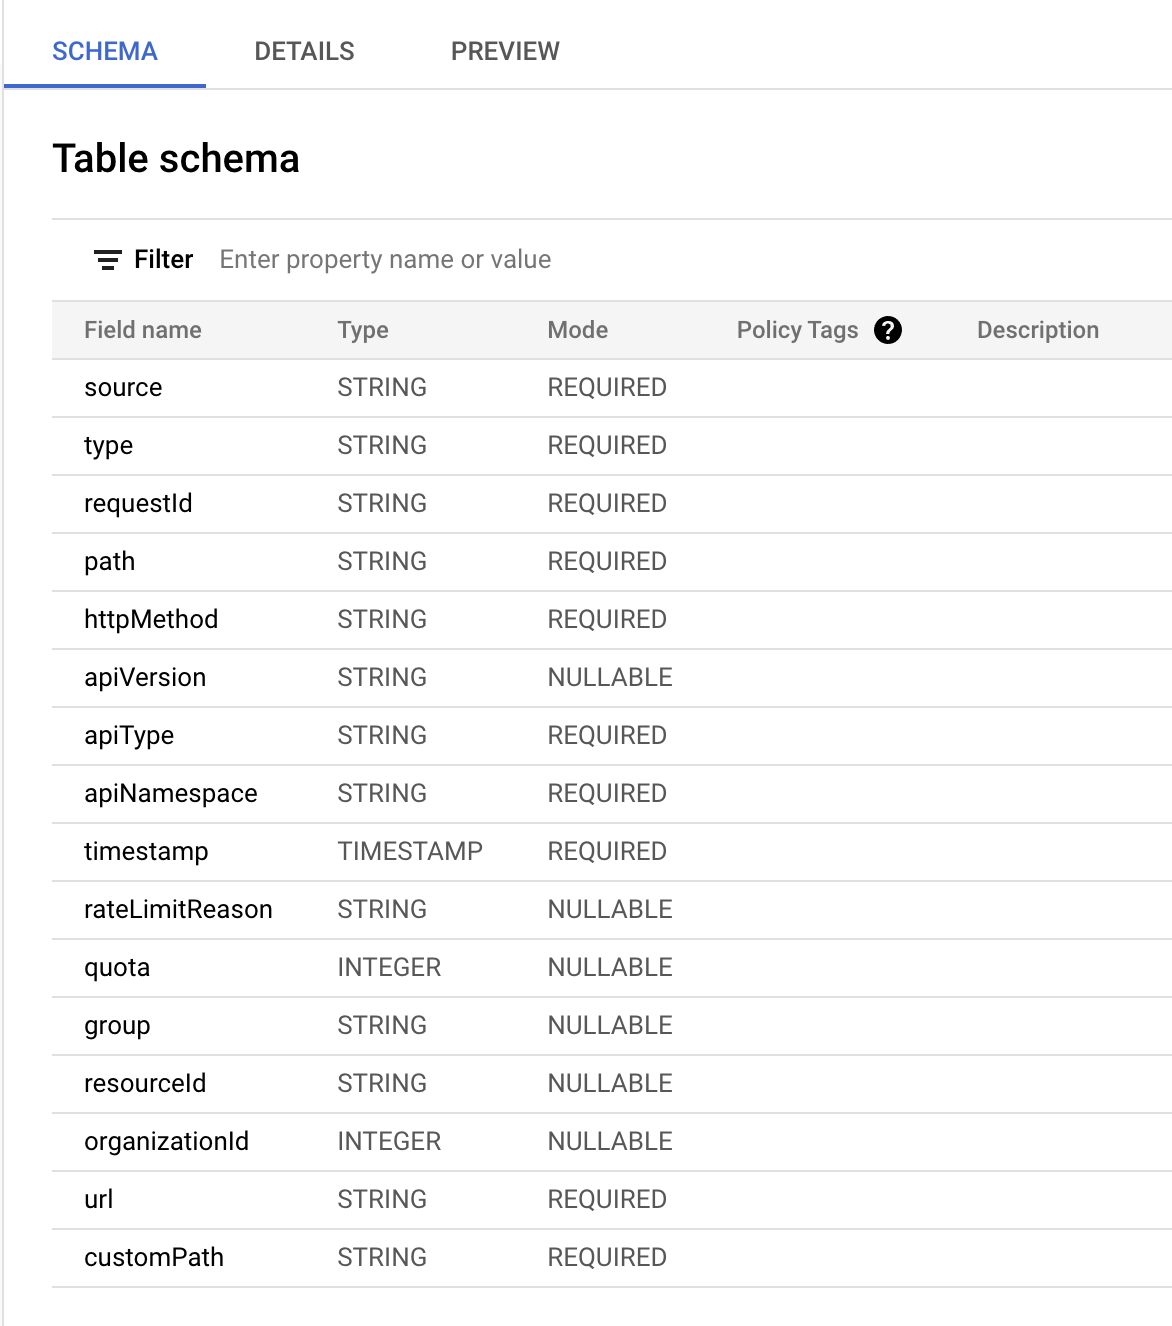
\includegraphics[scale=0.3]{src/thesis/img/technical-solution/bigquery-schema.png}
    \caption{Schema of the created BigQuery table}
    \label{fig:bigquery-schema}
\end{figure}

The next steps will be to implement the data gathering on the gateway microservice and create a log sink (section \ref{sec:log-sink}) for starting storing data on the warehouse.

\subsubsection{Event gathering implementation on Unity Services gateway}
\label{sec:event-gathering}

This section explains which concrete changes had been introduced on the Unity Services Gateway codebase to support the new events gathering. A diagram for this process can be observed on figure \ref{fig:event-gathering}.\\

\begin{figure}[h!]
    \centering
    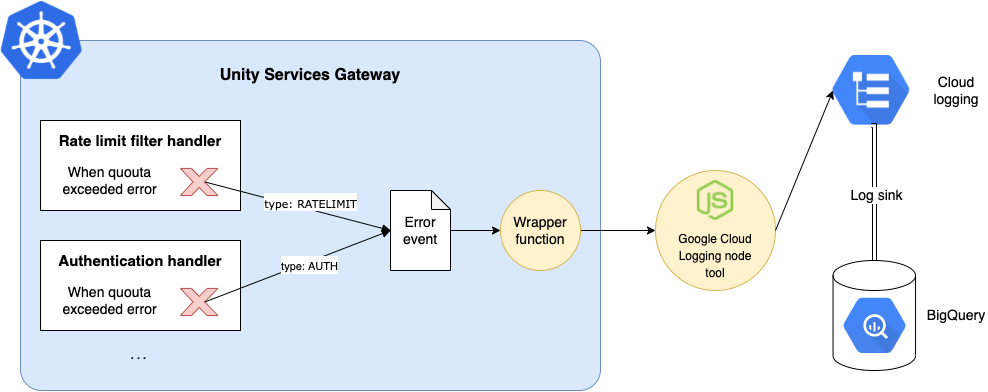
\includegraphics[scale=0.4]{src/thesis/img/technical-solution/events-gathering.png}
    \caption{Diagram that shows how the events gathering work on the Unity Services Gateway and how the log sink works}
    \label{fig:event-gathering}
\end{figure}

The first change introduced on the gateway consists of adding a wrapper JavaScript function to the Google Cloud Logger that will construct the event structure that BigQuery expects (explained in section \ref{sec:error-event-definition}). That function will be used instead of the current logger in the codebase where the events are triggered.The logger function is straightforward, it mainly matches the object that is given as a parameter, and then it enriches some fields from the request that it is receiving. Those parameters are the Organization ID obtained from the path parameter and the Request ID, injected by the gateway in an intermediate middleware. The code for the function can be seen at appendix \ref{apx:gateway-gathering}.\\

As stated before, only the rate-limiting events are considered; thus, only those events have to be logged for this iteration. This means the function that performs the rate limiter has to be modified to include the logging using the previous utility. It is first essential to explain how the rate limit quota is calculated, for doing that, a Redis database is set up with the Organization ID and a numeric value that increments when a new request is resolved. When the quota is exceeded, a new event is triggered containing the information if there were too many requests per 30 minutes or second.\\

Finally, it is relevant to state how the extensibility for this module will be done. If an additional field needs to be added to the database, then the logging function can be modified accordingly to contain it, and in the part of the codebase where that event is triggered, that logging function should be invoked. Apart from this, a default value should be set on this new field to ensure retro compatibility.

\subsubsection{Log sink configuration}
\label{sec:log-sink}

Section \ref{sec:event-gathering} explains that the events are collected using the standard Google Cloud logging tool on the Unity Services Gateway side. Still, for this project, it is not only needed to have the logs on the Google Cloud Logging, but it also needed to be persisted on a big data tool (in this case, BigQuery) for future analysis. GCP uses Sinks \cite{GCPSinks} to do this log routing and redirection, and this section explains how they were configured in this project.\\

As the organization is using Terraform for configuring all the infrastructure, for creating this sink, a new Terraform resource (with type \texttt{google\_logging\_project\_sink} \cite{TerraformGoogleSink}) has to be added. Then the configuration has to be applied to take effect. On Terraform, the structure for creating the log sink is as follows:\\

\begin{lstlisting}[language=json,firstnumber=1]
resource "google_logging_project_sink" "log_sink" {
  name                   = var.sink_name
  destination            = "bigquery.googleapis.com/projects/${google_bigquery_dataset.dataset.project}/datasets/${google_bigquery_dataset.dataset.dataset_id}"
  filter                 = var.filter
  unique_writer_identity = true

  bigquery_options {
    use_partitioned_tables = true
  }
}
\end{lstlisting}

As it can be seen, this code is parametrized, as many BigQuery log sinks are used across the organization. To create a new sink, a new module has to be created that extends this base code:\\

\begin{lstlisting}[language=json,firstnumber=1]
module "unity_services_gateway_metrics_log_sink" {
  source = "bigquery-logsink"

  dataset_id = "unity_services_gateway_metrics"
  sink_name  = "unity-services-gateway-metrics-stg-bigquery-log-sink"
  filter     = "resource.type=\"k8s_container\" AND (labels.k8s-pod/app=\"unity-services-gateway-public\" OR labels.k8s-pod/app=\"unity-services-gateway-internal\") AND jsonPayload.key=\"METRICS\""
}
\end{lstlisting}

This module extends the original log sink configuration, specifying a name for the log sink and the identifier for the BigQuery table where the log is going to be stored. One noticeable thing is that a filter is specified for distinguishing the logs containing the expected metrics. That is done by filtering only the records from the \texttt{unity-services-gateway-internal} or \texttt{unity-services-gateway-public} app, including the \texttt{"METRICS"} identifier.

\subsection{Error visualization dashboard}
\label{sec:visualization-dashboard}

%% Cover here the grafana dashboard implementation tool

%% - Cover the usage of the Grafana + BigQuery tool.
%% - Describe the different panels that had been developed.
%% - Persistance of the dashboard and deployment on every build.

This section covers the creation of a visualization tool for the high-level errors generated by the Unity Services Gateway and, therefore, how \textbf{Q3} is solved. It is composed of three subsections; the first one explains the integration tool used to connect Grafana with BigQuery, the second one explains the panels created for the dashboard, and the final one describes how the persistence of the continuous deployment had been done for it.

\subsubsection{BigQuery and Grafana connection}

One of the main characteristics of Grafana is that it is agnostic to the storage technology that is being used for the time series data that is going to be shown on the generated plots. This means that for adding different data sources, a connection has to be established between Grafana and the selected data storage technology, which in the case of this project is BigQuery. In that regard, two steps had to be followed for establishing that connection; the first one consists of installing the official Grafana plugin (\texttt{bigquery-grafana} \cite{GrafanaPlugin}) on the current instance of the company, and the second step is to add BigQuery as a data source so Grafana can access its data by using SQL statements.\\

\begin{figure}[h!]
    \centering
    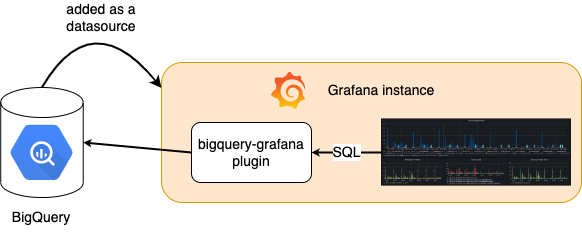
\includegraphics[scale=0.5]{src/thesis/img/technical-solution/grafana-connection.png}
    \caption{Diagram showing the connection between Grafana and Big Query}
    \label{fig:grafana-connection}
\end{figure}

In order to fulfill the first step, thus installing the plugin on the Grafana instance, the procedure consists of adding the URL and the variable that sets how the plugin should be loaded on the Helm chart of the Grafana instance. For doing that, the file \texttt{values.yaml} has to be modified in two sections, \texttt{plugins} and \texttt{grafana.ini}, adding the following values:\\

\begin{lstlisting}[language=json,firstnumber=1]
  plugins:
     - https://github.com/doitintl/bigquery-grafana/releases/download/2.0.3/doitintl-bigquery-datasource-2.0.3.zip;doit-bigquery-datasource

  grafana.ini:
    plugins:
      allow_loading_unsigned_plugins: doitintl-bigquery-datasource
\end{lstlisting}

On the \texttt{plugins} section, the URL of the official repository is specified alongside the desired version, so when loaded, the Grafana application will know where to download the plugin from. Additionally, the \texttt{grafana.ini} section specifies the name of the plugin to be loaded, in this case, \texttt{doitintl-bigquery-datasource}. After this configuration is applied and the Helm application is deployed, the plugin should be accessible from the Grafana instance. \\

The second step for establishing a connection between Grafana and BigQuery is adding it as a data source. As the infrastructure management of these project is using Terraform, adding a new data source for Grafana consists of adding the already existent BigQuery table as a Terraform resource \cite{TerraformResource}.\\

There are two steps for adding this resource on Terraform; first, the different configurations for BigQuery, are defined as Terraform locals on the terraform data sources configuration file. The objective is to avoid repetition on the creation of new resources while simplifying the addition of a new BigQuery data source (or even other types of data sources, such as Prometheus) to the infrastructure. The definition of the locals is as follows:\\

%% The real name of the project and the service account had been hidden for privacy reasons
\begin{lstlisting}[language=json,firstnumber=1]
locals {
  // some other datasources ...
  bigquery = {
    // some other BigQuery datasources ...
    "bigquery-unity-services-foundation-prd" = {
      "project"         = "gateway-metrics-ds"
      "service_account" = "gateway-metrics@iam.gserviceaccount.com"
    }
  }
}
\end{lstlisting}

After the local variables are added is time to create the BigQuery data source resource, which is specified as follows:\\

\begin{lstlisting}[language=json,firstnumber=1]
resource "grafana_data_source" "bigquery" {
 for_each = local.bigquery
 
 type = "doitintl-bigquery-datasource"
 name = each.key
 
 json_data {
     token_uri = "https://oauth2.googleapis.com/token"
     authentication_type = "jwt"
     default_project = each.value.project
     client_email = each.value.service_account
 }
}
\end{lstlisting}

The resource generation is generalized for each data source specified as locals (using a \texttt{for\_each}). Apart from that, there are two schema fields, \texttt{type}, and \texttt{name}. The first one defines the data source name extracted from the key of the locale, and the second one specifies the type determined by the Grafana plugin previously installed. Additionally, one meta-argument \cite{TerraformMeta} (\texttt{json\_data}) defines the data used when the current resource is created once the Terraform configuration is applied.\\

For managing the access to the BigQuery data source, the official JSON configuration accepts a \texttt{client\_mail} field to check the access rights. Nevertheless, this is matched to the \texttt{service\_account} field on the locale definition; this happens because the organization uses Role-Based Access Control to check the required permissions. It is relevant to mention that there is an additional process for creating a new service account for granting reading rights to the BigQuery data source, which is also done by creating another Terraform resource.

\subsubsection{Grafana dashboard}

In this section, it is going to be explained the handcrafted Grafana dashboard used for the visualization of the high-level errors that the gateway emits. This dashboard's objective is to effectively communicate those errors with the relevant stakeholders and establish the optimal way for visually representing those and consequently answering \textbf{Q3}.\\

One of the essential parts of this dashboard is the variables that will control the information that will be displayed on the panels. Variables work as follows: depending on the values selected, the events that match those values will be visualized on the boards. On this dashboard, six different variables are created (Figure \ref{fig:grafana-vars}).

\begin{figure}[h!]
    \centering
    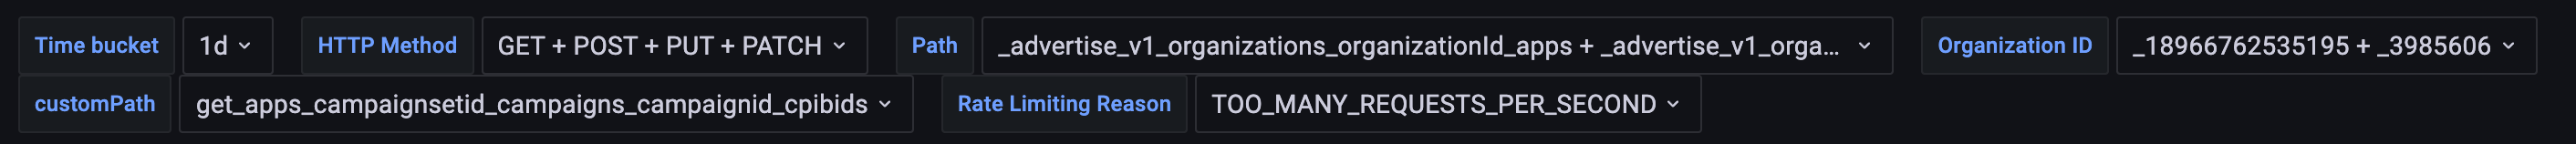
\includegraphics[scale=0.3]{src/thesis/img/technical-solution/grafana-dashboard/grafana-variables.png}
    \caption{Overview of the six Grafana variables created}
    \label{fig:grafana-vars}
\end{figure}

\begin{itemize}
    \item \textbf{Time interval}: this variable is not explicitly created for this project, but it is a default variable on Grafana. It defines the time range that will be selected for showing the time series data.
    \item \textbf{Time bucket}: It can be more understandable to show bucketed data instead of individual events when representing plots. This variable defines which is the time interval considered for those buckets.
    \item \textbf{HTTP method}: this variable defines the HTTP method of the gateway event that will be shown on the visualizations.
    \item \textbf{Path}: The path of the resource consumed which caused the gateway event to be triggered.
    \item \textbf{Organization ID}: The ID of the organization that triggered the gateway event.
    \item \textbf{Custom path}: this is a custom string that combines HTTP method and path, and it is used for visualization purposes.
    \item \textbf{Rate Limit reason}: it is essential to mention that at the moment, this dashboard is only visualizing rate limit events, even though it can be easily extended in the future. This variable represents which of the rate limit reasons is surpassed on the considered event.
\end{itemize}

It would not have been an extensible approach to manually insert the possible values for those variables, mainly because some of them, like the organization ID, could contain hundreds of possible values. In that regard, SQL was used for setting the possible values for them. The general structure for the SQL queries is the following:\\

% Again the real name of the table is hidden for confidentiality reasons.
\begin{lstlisting}[language=sql,firstnumber=1]
SELECT DISTINCT jsonPayload.variable_name
FROM `gateway_metrics_ds`

-- delimiter of the time range selected
WHERE `timestamp` BETWEEN TIMESTAMP_MILLIS($__from) and TIMESTAMP_MILLIS($__to)
  
-- set of common where clauses for variables
AND jsonPayload.source = "RATELIMITER"
AND jsonPayload.api_type = "public"
AND jsonPayload.api_namespace="advertise"

-- aditional WHERE for previous variables
-- e.g. for path variable
AND jsonPayload.http_method IN ($http_method)

ORDER BY jsonPayload.variable
\end{lstlisting}

On that query, the \texttt{SELECT DISTINCT} clause generates a list of possible values that the variables section of the Grafana dashboard can interpret. Furthermore, the variables are concatenated from left to right, so an extra \texttt{WHERE} clause is added in each query to set the previous variables' values.\\

In continuation with the explanation of the dashboard, the different panels that were created are going to be reviewed. The Grafana dashboard is divided into separate rows, and for each row, there is going to be a set of panels that share some characteristics.

\begin{figure}[h]
    \centering
    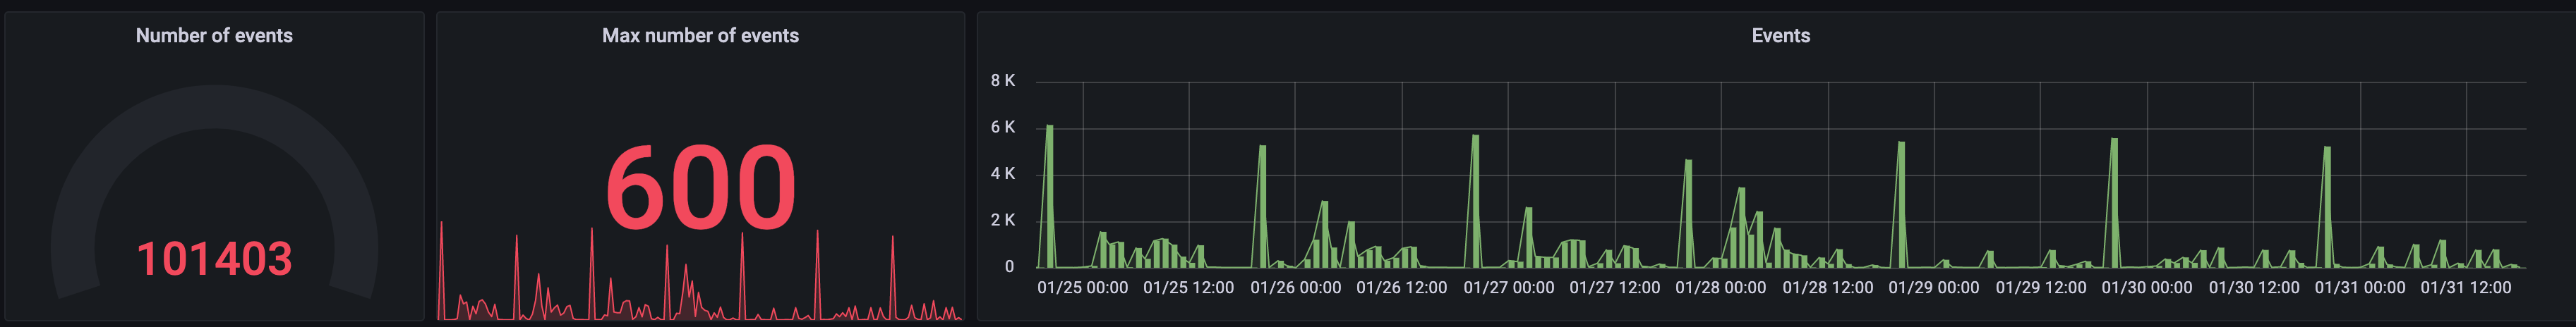
\includegraphics[scale=0.24]{src/thesis/img/technical-solution/grafana-dashboard/row-1.png}
    \caption{First row of the Grafana dashboard}
    \label{fig:grafana-row-1}
\end{figure}

The panels of the first row (Figure \ref{fig:grafana-row-1}) give general information about the number of events generated by the gateway. The left panel is a gauge type of plot that shows the total number of events considering all the selected variables. The central panel is a stat type of plot that offers the most significant spike in events, showing the maximum number registered on the specified bucket. Finally, the left one shows the total number of events disposed by the selected bucked on the chosen time range. To gather the data for those panels the same SQL statement is shared across them:\\

% Again the real name of the table is hidden for confidentiality reasons.
\begin{lstlisting}[language=sql,firstnumber=1]
SELECT 
  $__timeGroup(timestamp, $time_bucket),
  count(*) AS n_events
FROM 
  `gateway_metrics_ds`
WHERE 
  $__timeFilter(timestamp)
  -- ...
  -- all the additional WHERE clauses for each variable
GROUP BY 1
\end{lstlisting}

\begin{figure}[h]
    \centering
    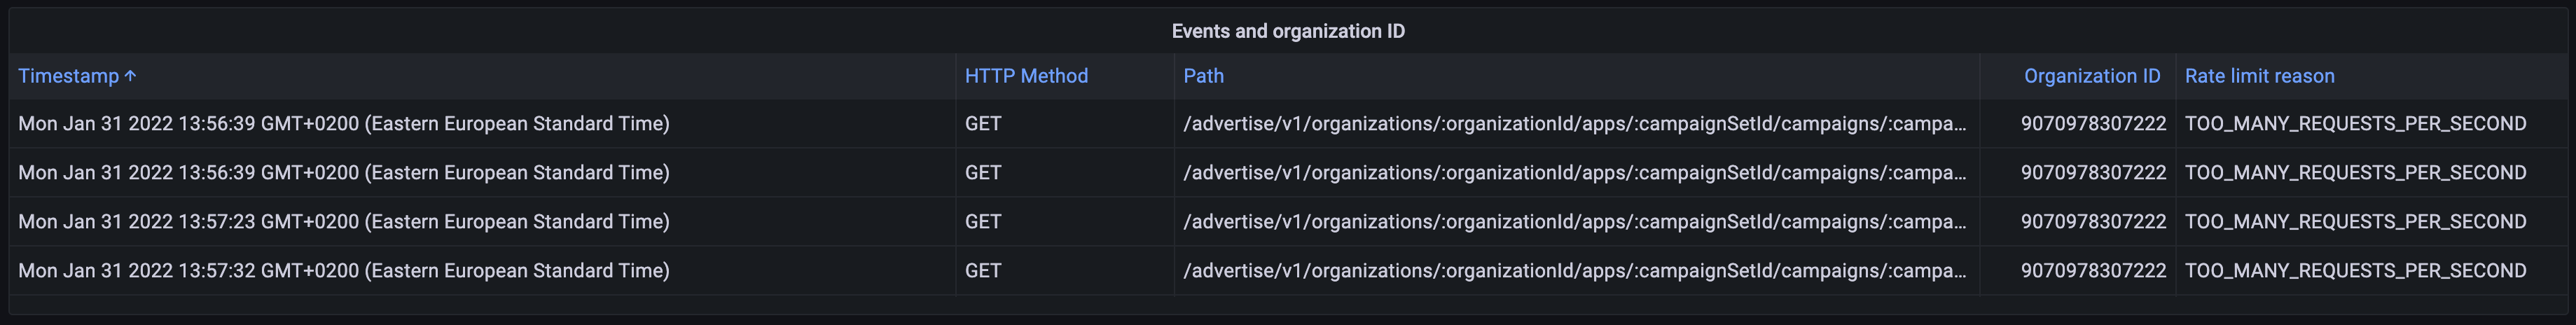
\includegraphics[scale=0.24]{src/thesis/img/technical-solution/grafana-dashboard/row-2.png}
    \caption{Panel of the dashboard showing the detailed information of the events}
    \label{fig:grafana-row-2}
\end{figure}

The second row (Figure \ref{fig:grafana-row-2}) is a table that offers more detailed information about the events in the selected period. The five columns of the table are timestamp, HTTP Method, path, organization ID, and rate limit reason. The primary purpose of this table is to offer a more detailed view that would make the identification of specific events faster.

\begin{figure}[h]
    \centering
    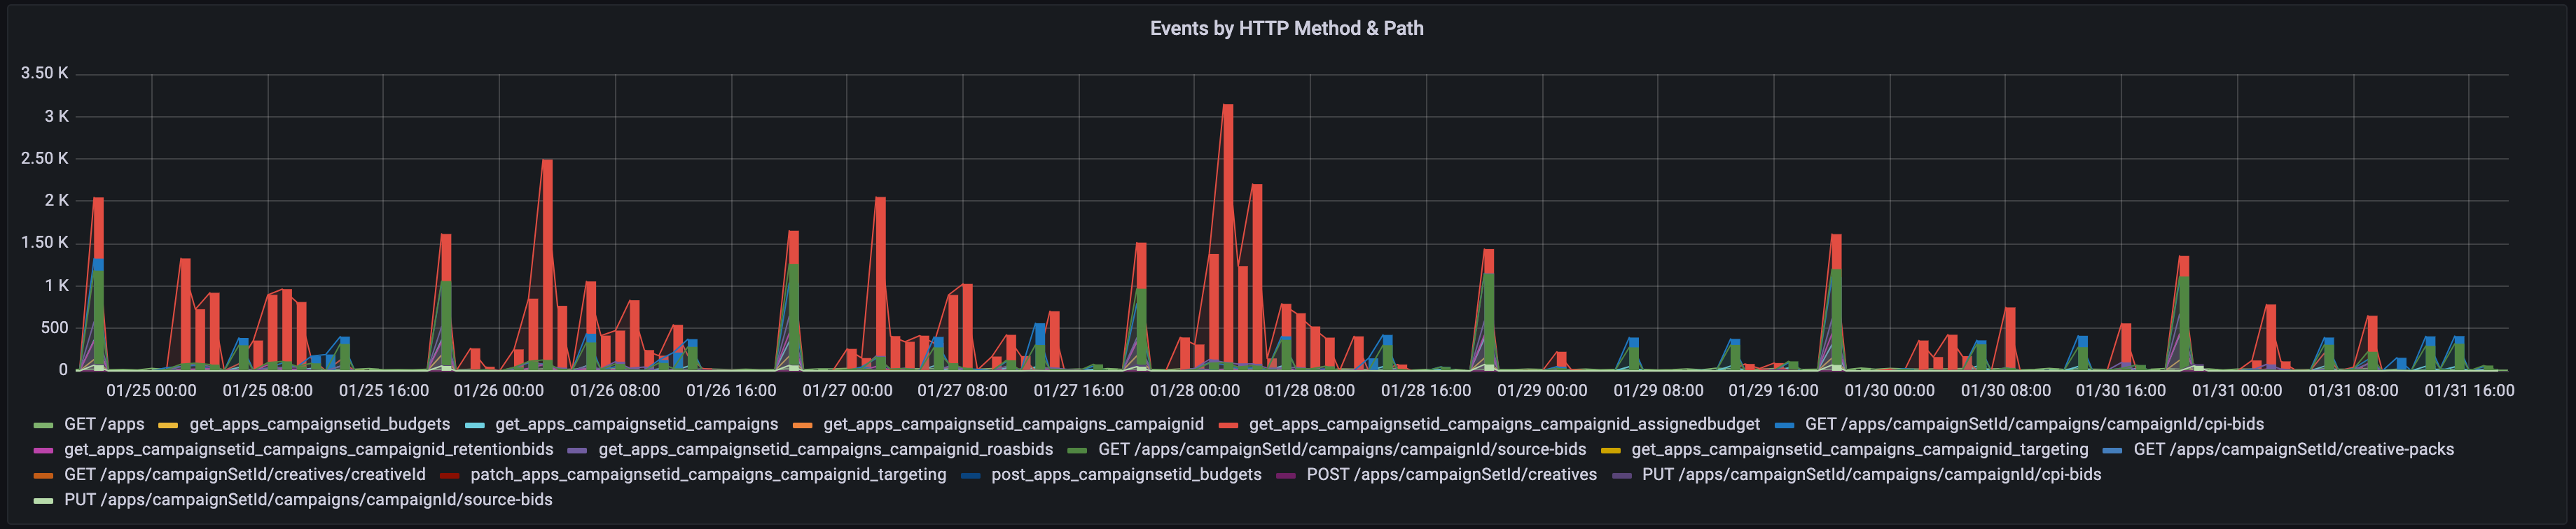
\includegraphics[scale=0.24]{src/thesis/img/technical-solution/grafana-dashboard/row-3.png}
    \caption{Panel showing the time series layout of the combination of HTTP method and path}
    \label{fig:grafana-row-3}
\end{figure}

The third row (Figure \ref{fig:grafana-row-3}) contains a time series panel showing the combination of HTTP method and path that triggered the gateway event. Previously, it was stated that the variable \textbf{Custom path} combines HTTP method and path into a single variable, and the primary purpose is to build this panel. The SQL statement to gather the data is the following:

\begin{lstlisting}[language=sql,firstnumber=1]
select *
from
(
  SELECT
    $__timeGroup(timestamp, $time_bucket),
    jsonPayload.custom_path
  FROM 
    `gateway_metrics_ds`
  WHERE 
    $__timeFilter(timestamp)
    -- ...
    -- all the additional WHERE clauses for each variable
) d
pivot
(
  count(custom_path)
  for custom_path in (
    $custom_path
  )
) piv
order by time
\end{lstlisting}

As can be seen, the \texttt{PIVOT} clause transforms the different rows into columns and builds the time series data displayed on the plot. Unfortunately, in this process, the two variables can not be combined, so this is why a variable that contains both values has to be created.\\

\begin{figure}[h]
    \centering
    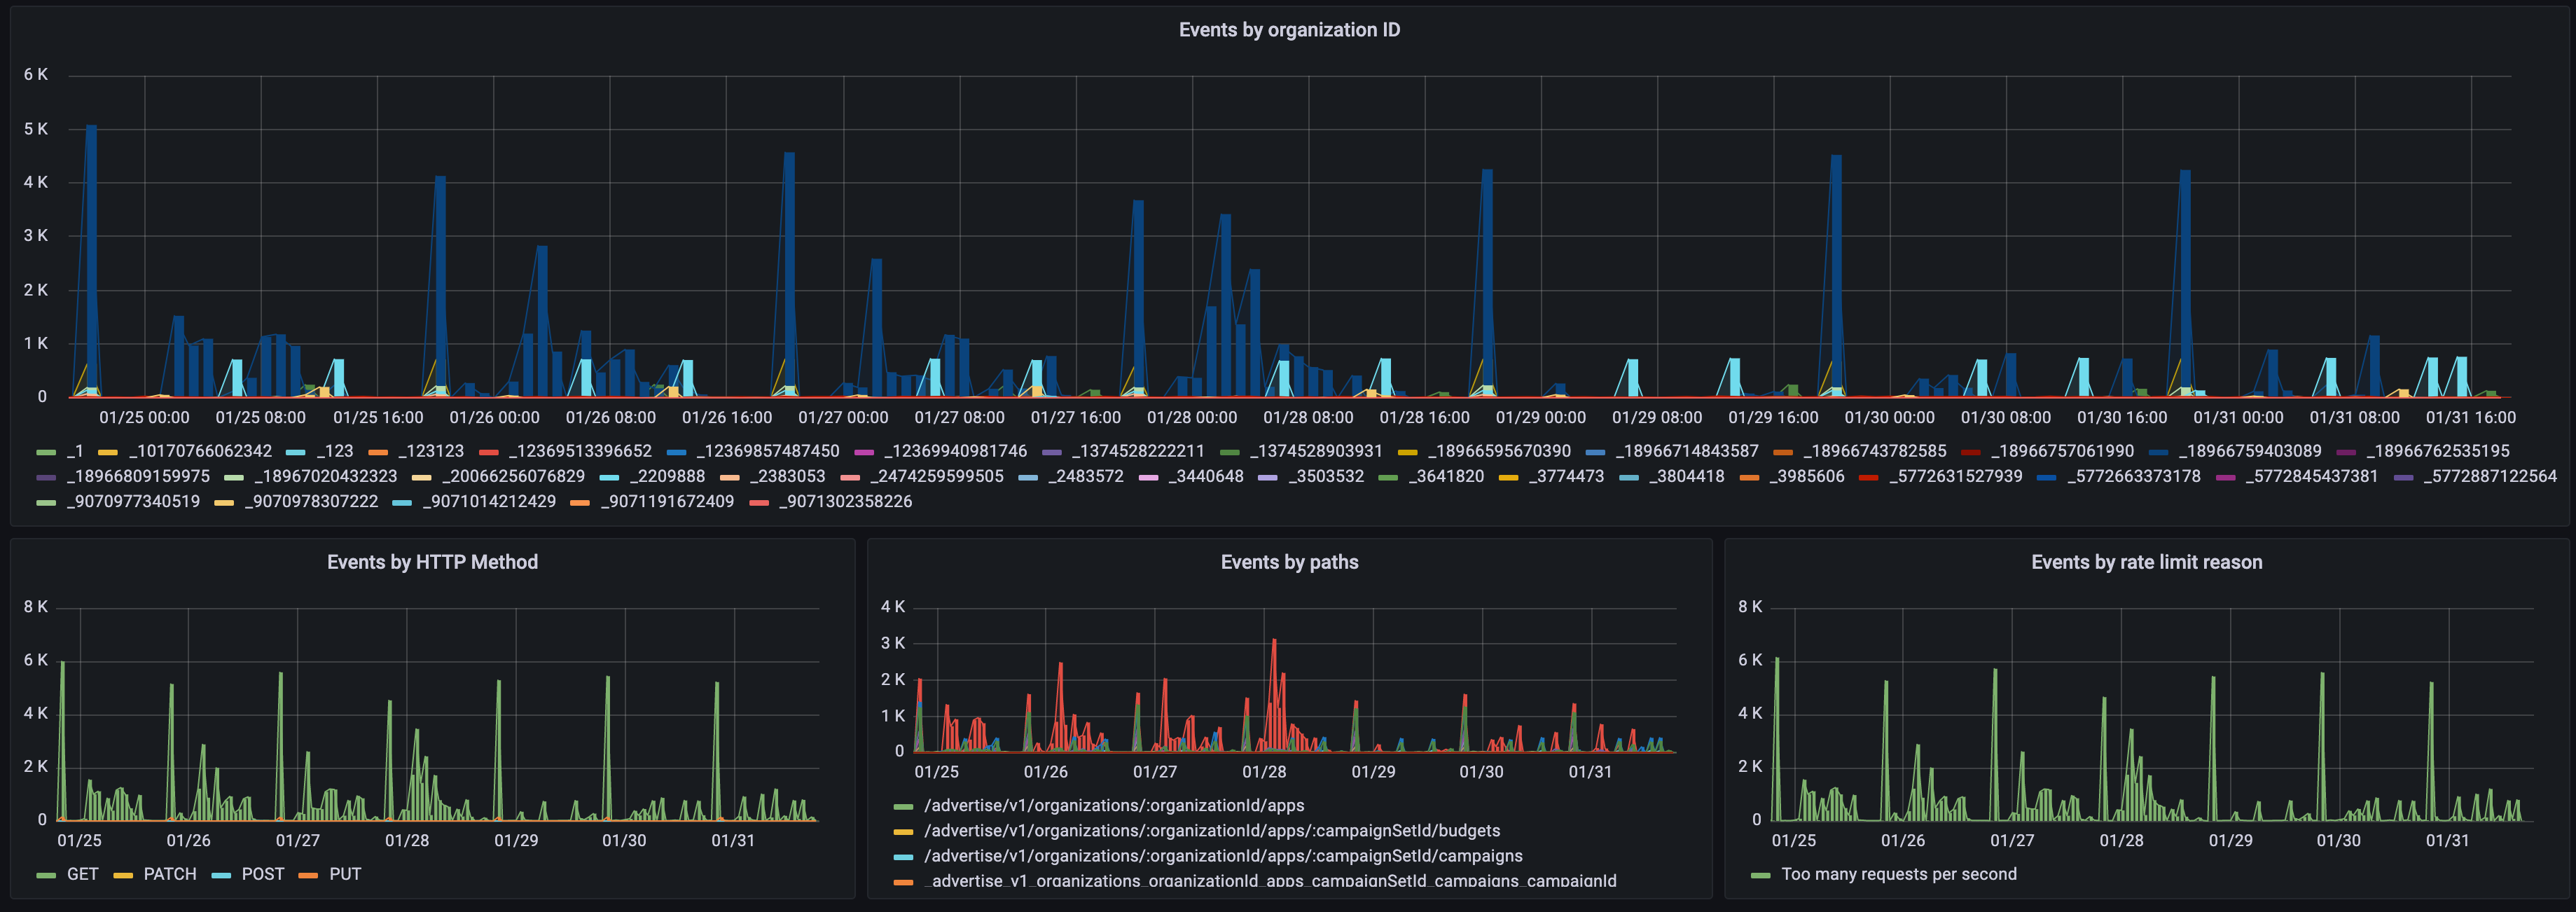
\includegraphics[scale=0.24]{src/thesis/img/technical-solution/grafana-dashboard/row-4.png}
    \caption{Panel showing the time series layout divided into the different possible values of the variables}
    \label{fig:grafana-row-4}
\end{figure}

Finally, the fourth and fifth rows (Figure \ref{fig:grafana-row-4}) contain different panels showing the distribution of previously explained variables, like the events divided by other Organization IDs, HTTP Method, or path. One thing to notice is that the last panel shows the events by different rate limit reasons, and this is the only panel specific to rate limit events. The example SQL statement used for building those panels is the one used for the variable \texttt{rate\_limit\_reason}, and it is equivalent to the others, but only changing the variable name.\\

\begin{lstlisting}[language=sql,firstnumber=1]
select *
from
(
  SELECT
    $__timeGroup(timestamp, $time_bucket),
    jsonPayload.rate_limit_reason
  FROM 
    `gateway_metrics_ds`
  WHERE 
    $__timeFilter(timestamp)
    -- ...
    -- all the additional WHERE clauses for each variable
) d
pivot
(
  count(rate_limit_reason)
  for rate_limit_reason in (
    $rate_limiting_reason
  )
) piv
order by time
\end{lstlisting}

Finally, it is essential to notice that the extensibility of these panels is straightforward. If a new field is introduced on the gateway event (section \ref{sec:error-event-definition}), the only change on the dashboard side would be to duplicate one of the last panels and change the variable name on the SQL statement.

\subsubsection{Grafana dashboard persistence}

In this last section, it is going to be explained how the Grafana dashboard is persisted and correctly versioned. The objective is to have a way to recover the dashboard if something happens and not only rely on click-opts to create and save it. Additionally, the dashboard will be stored on a VSC so it can be versioned; thus, team members can review its new changes before deploying it.\\

Once the dashboard is created, the next step is to generate a JSON file in the Grafana format \cite{GrafanaJson} through the UI. That JSON Document will be persisted in the private repository of the project. For doing that, a PR has to be created containing the copied file under the \texttt{monitoring/dashboard} directory. That particular file location is chosen because a company-wide automation deploys the dashboards located under that folder for each repository.\\

After this first version is created, future changes or maintenance will follow this procedure: import the JSON file into Grafana, make the changes that are required, export the new JSON file replacing the old one in the repository, and finally create a new PR that explains the differences and that the team that owns the service has to review before being merged and deployed.

\clearpage
\section{Evaluation}
\label{sec:evaluation}

This section will cover the evaluation of the proposed framework. Two sub-sections are introduced for that purpose; the first will cover the internal evaluation techniques used to verify that it fulfilled the expectations; the second will compare the proposed framework against two of the most relevant tools already present in the industry.

\subsection{Internal evaluation of the proposed framework}
% The different parts of the framework that are evaluated are the following:
% - Evaluation of the event gathering code (using jest).
% - Evaluation of the storage selection. Explain that there is the staging and the production data storage and that an script was created in order to inject data and try different configurations.
% - For evaluating the Grafana dashboard we also created two instances.
% - Create a tests script that will trigger some events on the gateway side and that was executed for the staging deployment
% - Internal release with continuous feedback from the stakholders (APIs team, Gateway team and product managers).

This section will cover the different steps used internally for verifying the proper functioning of the proposed framework, not only from the technical point of view on the different phases but also from the expected requirements point of view.

\subsubsection{Event gathering phase evaluation}
\label{sec:event-gathering-eval}

This first subsection covers the evaluation of the event gathering phase, which was initially introduced in section \ref{sec:event-gathering}. As explained before, this phase consisted of creating a wrapper logging function on the Unity Services Gateway codebase that will construct the event with the expected format, emitted to BigQuery afterward.\\

For evaluating this logging function and correctly testing if the event mapping was done as expected, the selected methodology was doing a battery of unit tests that will be part of a CI pipeline that ensures the correct functioning of the service. The chosen library for this purpose was Jest, as it is already used on other parts of the service. The complete code of the test can be observed in appendix \ref{apx:jest-eval}.

\subsubsection{Data pipeline, storage and visualization dashboard evaluation}

The data pipeline, data storage, and error visualization dashboard were evaluated in several steps. One of the main characteristics of this evaluation is that for having a safe sandbox where to do testing for the development of this project and in the future, two different environments, staging, and production, were created. Production will contain the data and instances that will be delivered to the clients, and staging will be an exact clone where testing procedures should be executed.\\

One of the first relevant tests was if the data was stored correctly in BigQuery. For doing that, a script that generated fake events was placed and connected to the data store in staging. That script inserted 10.000 events with the structure introduced in section \ref{sec:error-event-definition} on the staging instance of the dataset. This method allowed us to test that the event´s format was correct, and also, the fake data introduced can be used for testing the dashboards visualization afterward.\\

Finally, for evaluating the visualization dashboard, there were two instances of it created in Grafana. One was extracting the data from the production database and the other from the staging database. The manual test done in that regard was checking that the data inserted before on the staging data source could be visualized as expected on the staging dashboard. Apart from that, the query structure was confronted with the BigQuery console results.

\subsubsection{End to end evaluation}
\label{sec:e2e-eval}

The end-to-end evaluation consisted of deliberately generating error events on the Gateway service to check if there are correctly stored on the data source and visualized in the dashboard afterward. This step can only be done after deploying the event-gathering code on the staging environment and applying the terraform configuration for the log sinks and Grafana.\\

As it was stated in section \ref{sec:error-event-definition}, the high-level events will only include rate-limiting in this first iteration of the framework. In that sense, to test if the errors are correctly stored and visualized, they must first be generated. A new bash script was created that will call different endpoints in a loop a certain number of times over the expected quota, thus causing the expected errors. The script can be observed in appendix \ref{apx:bash-script}.\\

After creating and calling that script, the resulting events were observed on BigQuery and correctly visualized in the dashboard; thus, the framework could be safely deployed in the production environment.

\subsection{Comparison with state-of-the-art gateway frameworks}
\label{sec:gateways-comparison}

In this section, the proposed framework will be compared to the two integral gateway solutions that are standards in the industry: The Gateway by Kong technologies and the Zuul gateway by Netflix, already introduced in section \ref{sec:industry-gateways}. Those two examples are out-of-the-box integral gateway solutions, so they present more functionalities than the proposed framework; therefore, they will be compared by the expected criteria exposed in section \ref{sec:req-analysis}. The primary purpose of this comparison is to evaluate if the industry solutions already fulfill these criteria and to assess this proposed framework in conjunction with the Unity Services Gateway.

\subsubsection{Frameworks comparison}

The three solutions will be compared using four criteria to determine if the expected outcomes defined in section \ref{sec:req-analysis} are achieved.

\subsubsection*{C1 - High-level responsibilities matching to individual routes}
In this criterion, the frameworks will be evaluated concerning if they have a way to match the high-level responsibilities that they have to the routes that the gateway is exposing. The comparison is the following:

\begin{itemize}
    \item \textbf{Kong}: This gateway has a minimalistic approach when defining the responsibilities it will take, as it is plugin-based. The plugins must be installed per different instances, and many of them are premium features. There are two options for defining the responsibilities that each route will take: by using the administrator UI, relying on click-opts for introducing the data, or doing a REST API call once the service is deployed.
    \item \textbf{Zuul}: There is a clear definition of the responsibilities on this gateway, but matching them to the routes is done by using code, as the routes are defined using Java classes.
    \item \textbf{Proposed framework}: The routes definition format is explained in section \ref{sec:gateway-configuration-file}.
\end{itemize}

As it can be seen, the only gateway that provides file-based configuration is the proposed framework. It might seem a disadvantage as the format is more straightforward if done through a UI. Nevertheless, using a file adds the option of introducing new changes to the structure and CI/CD capabilities.

\subsubsection*{C2 - Error format definition}
This criterion refers to the possibility of adding enriched fields to the events gathered on the gateway side, defining our format. The comparison is the following:

\begin{itemize}
    \item \textbf{Kong}: As this framework is an out-of-the-box solution, the time needed for the configuration is effortless, but the configuration possibilities are limited. In this case, there is no way to enrich the error fields and emit them to a secondary stream.
    \item \textbf{Zuul}: This framework allows error configuration and custom handling by catching the error on the codebase and adding an extra mapping and emission step.
    \item \textbf{Proposed framework}: Events are defined with the relevant fields to persist and be visualized afterward (section \ref{sec:error-event-definition}) and gathered on the codebase (section \ref{sec:event-gathering}).
\end{itemize}

\subsubsection*{C3 - Data storage selection}

This criterion refers to the existence of data pipelines and data storage technology for the persistence of the event that will ensure the proper visualization and discovery afterward.

\begin{itemize}
    \item \textbf{Kong}: This solution provides Cassandra and PostgreSQL for storing rate-limiting and authentication events that the gateway emits.
    \item \textbf{Zuul}: This framework does not offer any custom integration to store data events. As it is a library module, all the integration has to be custom-built, which can be equivalent effort as the proposed framework, but in a language (Java) that does not fit directly on the company's technical stack.
    \item \textbf{Proposed framework}: Events are stored on BigQuery, and the data pipeline is defined as a GCP sink (section \ref{sec:log-sink}).
\end{itemize}

\subsubsection*{C4 - Visualization of high-level errors}

This criterion sets the existence of a visualization tool that allows the stakeholders to visualize the high-level error events of the gateway simply. In that regard, of the compared frameworks, only the proposed solution includes this visualization tool, explained in section \ref{sec:visualization-dashboard}.

\subsubsection{Frameworks comparison conclusions}

% Please add the following required packages to your document preamble:
% \usepackage[normalem]{ulem}
% \useunder{\uline}{\ul}{}
\begin{table}[h]
\begin{tabular}{|l|l|l|l|l|}
\hline
                  & \multicolumn{1}{c|}{C1} & \multicolumn{1}{c|}{C2} & \multicolumn{1}{c|}{C3}        & \multicolumn{1}{c|}{C4} \\ \hline
\hline
Kong              & Yes - with UI           & No                      & Yes - Cassandra and PostgreSQL & No                      \\ \hline
Zuul              & Yes - with code         & Yes                     & No                             & No                      \\ \hline
\textbf{Proposed solution} & Yes - with file         & Yes                     & Yes - BigQuery                 & Yes                     \\ \hline
\end{tabular}
\caption{Framework comparison table}
\label{tab:frameworks}
\end{table}

Table \ref{tab:frameworks} summarizes the comparison between the different frameworks. The conclusion that can be extracted is that even though Kong or Zuul are considered industry standards and are very competent products, they do not provide an automatic solution for the visualization and storing of the high-level events of the gateway.

\clearpage
\section{Conclusions}
\label{sec:consclussion}

%% This part is almost the last one to write, basically write some pages of conclussions, and offer future work

%% For future work basically it can be checked if there is something on the backlog.

%% Focus conclussion on an adoption analysis for the three types of organizations: startups, midsize organizations and large organizations.

In recent years, there has been an increase in the adoption of microservices architectures by extensive and well-established companies and small startups. On many of them, the amount and complexity of their architecture are so significant that they had to adopt patterns like DOMA, creating a gateway that allows them to simplify the operations that they had spread across many microservices. This thesis aims to offer a framework for developing and monitoring the high-level errors that those gateways are producing and giving procedures on how to increase their visibility of them across different teams.\\

The work developed during this thesis gave valuable insights that can be applied to any organization facing the same challenges that Unity Technologies. But it is remarkable to mention that this project is done within a multinational organization. Thus, the knowledge might not be applied in the same way for organizations of different sizes. This is why these conclusions might be divided to give insights depending on the organization's scale.

\subsubsection*{Startups}
On startups, the main goal is to develop the business's value proposition and give worth to the final customers. In those organizations, the number of employees is usually small, so there are not enough resources for implementing internal tools like the one proposed in this project.\\

The software architecture is usually monolithic or just a few microservices on these businesses. Therefore, as they are not running a DOMA, they are not the target of this project. Nevertheless, in the initial stages of software design is always beneficial to take into consideration that the architecture might change and scale in the future, and they might find the necessity of adopting a gateway after that initial stage.

\subsubsection*{Medium-sized enterprises}
Medium-sized enterprises have between 50 and 250 employees. If they are software-based, usually that means that they are running more than 50 microservices. In that case, probably the need for a standard gateway for the microservices has already arisen.\\

In that case, the most crucial step is defining how the format will be for determining the routes that the gateway will expose to the public and how to implement the high-level responsibilities. Considering this, one sensible approach will be to select one of the existing industry-standard solutions for the gateway (section CITE-SECTION), as it will dramatically reduce the implementation and maintenance time. One possible solution about the monitoring of it will be to adapt the knowledge exposed in the technical solution of this thesis (section CITE-SECTION) to the particular case of the gateway technology that they are running.

\subsubsection*{International enterprises}
On international enterprises with hundreds or thousands of employees and possibly microservices running, the most sensible approach will be to adopt a DOMA architecture while maintaining a gateway that will be the starting point of one or several domains. This is the case with Unity technologies or Uber.\\

This project makes most of the sense on those types of organizations, as different teams probably depend on others, working in various locations and times zones. In that case, visibility of the business logic is crucial, and monitoring the high-level gateway errors becomes very significant.

\subsection{Future work}
Different improvement ideas or future work that can be done on this topic are introduced in this section.\\

The first one is about the different types of errors that were mapped. As it was stated in section CITE-SECTION, for this project, only rate-limiting responsibility is considered for the monitoring; this is because it was the error that project managers and teams were more worried about. Nevertheless, other types of errors can be handled, and that can be done by extending the error type and using the custom function introduced in section CITE-SECTION.\\

The second improvement idea will be to create a gateway composable logic tool. Having the standard defined in section CITE-SECTION, the next step can be to create a solution that injects the handling of those high-level responsibilities on the gateway at execution time to minimize the effort for defining new routes and resources.\\

Finally, the last improvement idea will be to pack this knowledge into a fully-extendable tool that can be used in standard gateway solutions like Kong. For doing that, some pieces of this software should be re-written to ensure compatibility with the gateway solution that it is intended to be extended.

\clearpage
\thesisbibliography

\bibliographystyle{plain}
\bibliography{bibliography}

\clearpage
\thesisappendix

\section{Appendix 1}
\label{apx:gateway-gathering}

This appendix contains the code for the event gathering on the Unity Services Gateway:

\begin{lstlisting}[language=JavaScript,firstnumber=1]
const { logger } = require('@unity/node-monitoring');
function log(req,
  {
    quota,
    source,
    type,
    apiVersion,
    apiNamespace,
    rateLimitReason,
    group,
    resourceId,
  },
) {
  const organizationId = req.params?.organizationId ?? null;
  const requestId = req?.context?.id ?? '';
  const apiType = process.env.API_MODE ?? '';
  const event = {
    key: 'METRICS',
    path: req.route.path,
    url: req.url,
    httpMethod: req.method,
    customPath: `${req.method}_${req.route.path}`,
    source,
    type,
    apiVersion,
    apiNamespace,
    rateLimitReason,
    group,
    resourceId,
    apiType,
    requestId,
    organizationId,
    quota,
  };

  logger.log(event);
}
module.exports = { log };
\end{lstlisting}

\clearpage
\section{Appendix 2}
\label{apx:jest-eval}

This appendix contains the code for the test case written in JavaScript using the framework Jest for evaluating the event gathering function on the Unity Services Gateway (section \ref{sec:event-gathering-eval}).

\begin{lstlisting}[language=JavaScript,firstnumber=1]
const { logger } = require('../../monitor');
const { log } = require('./metrics');

describe('metrics', () => {
  let req;

  beforeEach(() => {
    jest.clearAllMocks();
    jest.spyOn(logger, 'log');
    req = {
      route: {
        path: '/url/:organizationId',
      },
      url: '/url/123',
      method: 'get',
      params: {
        organizationId: 123,
      },
      context: {
        id: 'abc-123',
      },
    };
  });

  it('should call logger one time', async () => {
    log(req, {});
    expect(logger.log).toHaveBeenCalledTimes(1);
  });

  it('should call logger with correct data', async () => {
    log(req, {
      quota: 10,
      source: 'RATELIMITER',
      type: 'QUOTA_EXCEEDED',
      apiVersion: 1,
      apiNamespace: 'advertise',
      rateLimitReason: 'TOO_MANY_REQUESTS_PER_SECOND',
      group: 'group-123',
      resourceId: '*',
      customPath: 'A-01:{#\\.}a/b',
    });

    expect(logger.log).toHaveBeenCalledWith({
      key: 'METRICS',
      path: '/url/:organizationId',
      url: '/url/123',
      httpMethod: 'get',
      time: expect.any(String),
      source: 'RATELIMITER',
      type: 'QUOTA_EXCEEDED',
      apiVersion: 1,
      apiNamespace: 'advertise',
      rateLimitReason: 'TOO_MANY_REQUESTS_PER_SECOND',
      group: 'group-123',
      resourceId: '*',
      apiType: '',
      requestId: 'abc-123',
      organizationId: 123,
      quota: 10,
      severity: 'info',
      customPath: 'a01a_b',
    });
  });
});
\end{lstlisting}

Two test cases had been included, the first one tests if the Google Logger function had been called only once and the second one tests if the mapped event matches the expected structure.

\clearpage
\section{Appendix 3}
\label{apx:bash-script}

This appendix contains the script used for triggering the rate limiting events on several endpoints, introduced on section \ref{sec:e2e-eval}.

\begin{lstlisting}[language=sql,firstnumber=1]
for i in {1..4010}
do
   curl --request GET \
  --url https://services.api.unity.com/advertise/v1/organizations/:organizationId/apps/ \
  --header 'Authorization: Basic <service-account>'
  
  curl --request GET \
  --url https://services.api.unity.com/advertise/v1/organizations/:organizationId/apps/:appId/campaigns \
  --header 'Authorization: Basic <service-account>'
  
  curl --request GET \
  --url https://services.api.unity.com/advertise/v1/organizations/:organizationId/apps/:appId/campaigns/:campaignId/budget \
  --header 'Authorization: Basic <service-account>'
done
\end{lstlisting}

Inside a loop that intends to exceed the established quota of 4000 calls per 30 minutes there are three calls to different endpoints. The concrete parameters for the endpoint are not included for privacy concerns.

\clearpage

\end{document}